\documentclass[12pt, letterpaper]{article}
\usepackage{graphicx} % Required for inserting images
\usepackage{hyperref}
\usepackage{listings}
\usepackage{amssymb}
\usepackage{amsmath}
\usepackage[english]{babel}
\usepackage{mathtools}
\usepackage[table,xcdraw]{xcolor}
\definecolor{light-gray}{gray}{0.95}
\definecolor{sap}{RGB}{130, 36, 51}
\usepackage[paper=a4paper,left=20mm,right=20mm,bottom=25mm,top=25mm]{geometry}
\newcommand{\code}[1]{\colorbox{light-gray}{\texttt{#1}}}
\newcommand{\codee}[1]{\colorbox{white}{\texttt{#1}}}
\newcommand{\acc}{\\\hphantom{}\\}
\newcommand{\dete}{{\rightarrow}}
\newcommand{\boxedMath}[1]{\begin{tabular}{|c|}\hline \texttt{#1} \\ \hline\end{tabular} :}
\title{Basi di Dati 1}
\author{Marco Casu}
\date{\vspace{-5ex}}
\begin{document}



\maketitle
\begin{figure}[h]
    \centering{
    
\includegraphics[width=0.85\textwidth ]{images/cop.png}
    }
\end{figure}
\newpage 
\tableofcontents
\newpage
\section{Introduzione}
L'informazione memorizzata nei sistemi elettronici può essere di due tipi, \textbf{strutturata}
e \textbf{non strutturata}. In questo corso ci occuperemo dell'informazion strutturata, ossia composta da 
oggetti matematici ben definiti. Un \textbf{sistema informativo} connette e contiene le informazioni,
alla quale si può accedere da diversi componenti. Si prenda come esempio di sistema informativo l'archivio
fisico dei documenti (ossia i dati) di una azienda, ad esso, possono accedere i vari reparti, come la sezione 
commercio o le risorse umane, ognuno ha a disposizione l'accesso ad un determinato sotto-insieme di dati (permessi).
Prima di adoperare i sistemi informativi, ogni reparto aveva il suo personale archivio, ciò faceva si che molti dei dati
fossero duplicati e presenti per più reparti, causando un elevata \textbf{ridondanza} di dati. Inoltre, due dati da 2 archivi
diversi potrebbero dipendere tra loro. È quindi importante mantenere l'informazione \textbf{centralizzata}.
I dati vanno organizzati, gestiti, e regolamentati da permessi di accesso a secondo dell'utente che vuole accedervi.
\\\\Un sistema informativo è composto dai seguenti componenti : 
\begin{itemize}
    \item Database (DB)
    \item Database Managment System (DBSM) - Ossia il software per il mantenimento dei dati  
    \item Application Software
    \item Computer Hardware - La memoria nella quale è contenuto
\end{itemize}
È importante mantenere una visione astratta del modello di sistema informativo, che sia indipendente
dall'hardware in uso. Fissiamo un modello che utilizzi tipi di dati che non possano variare nel tempo,
strutturati in maniera completa, è necessario pensare ad un metodo formale per organizzare i dati.
Vogliamo farlo in un ambiente condiviso, preoccupandoci quindi di quali e quanti dati vengono condivisi condivisi
con i singoli utenti, che avranno permessi diversi e potranno accedere a dati diversi (ad esempio, uno studente può
accedere ai suoi esami registrati, ma non a quelli degl altri). Inolte bisogna anche amministrare i metodi
con cui si accede ai dati, preoccupandoci della concorrenza (accedere allo stesso dato nello stesso momento).
I dati vengono organizzati in maniera omogenea, esiste un tipo di dato per descrivere un entità (ad esempio uno studente),
e tutte le volte che si vuole immagazinare nel sistema uno studente, bisogna ricorrere allo stesso tipo di dato.
L'informazione viene rappresentata da un aggregamento di più dati \textit{grezzi}, ossia, rispettivamente la stringa
 "\textit{Maurizio Ernesti}" e l'intero "3761523746", insieme rappresentano l'informazione di un 
 professore (nome, cognome e numero di telefono).\\\\
 Il modello è il modo in cui decidiamo di organizzare e collegare i dati, esistono modelli \textbf{logici}, 
 indipendenti dalla struttura fisica, come il \textbf{modello relazionale}, ed esistono modelli \textbf{concettuali},
 ossia rappresentazioni ancora più astratte indipendenti dal modello logico, i primi modelli sono stati introdotti
 negli anni 60.
 \\\\
 \begin{minipage}{0.16\textwidth}
    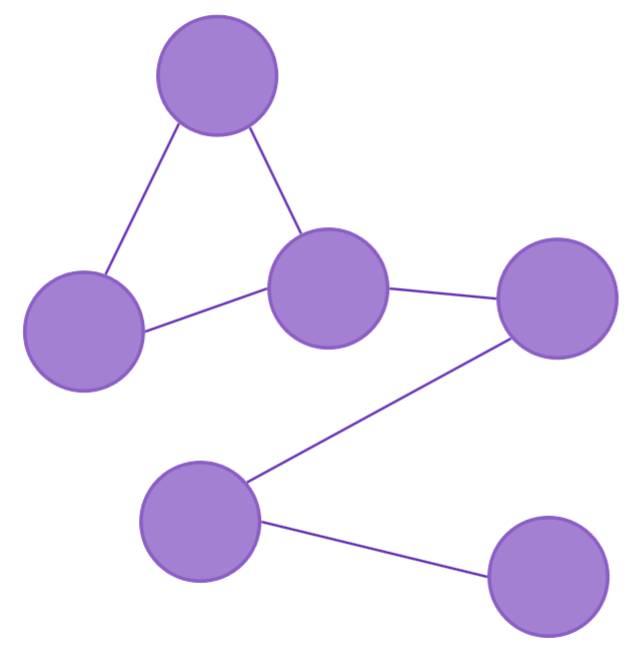
\includegraphics[width=\linewidth]{images/GrafoViola.png}
    \end{minipage}
    \begin{minipage}{0.8\textwidth}\raggedright
        un esempio è il modello \textit{Mesh}, rappresentato con un grafo, dove i nodi sono i dati (i record), e
        gli archi le loro relazioni.
    \end{minipage}
    \noindent
    \\\\
In questo modello i collegamenti sono esplicitati fisicamente (possiamo immaginare con dei puntatori), i modelli
relazionali, diversamente, hanno relazioni rappresentate implicitamente dai valori stessi che contengono.
\\

\centering
\begin{tabular}{|l|l|l|r|}
    \hline
\multicolumn{4}{|c|}{\textbf{Studenti}}\\
    \hline
    Matricola & Cognome & Nome & Compleanno\\
    \hline
    276545 & Gialli & Lucia & 25/11/1980\\
    \hline
    176515 & Rossi & Mario & 13/09/1982\\
    \hline
    348191 & Verdi & Andrea & 04/07/1981\\
    \hline
    \end{tabular}
\begin{tabular}{|l|l|l|r|}
    \hline
\multicolumn{3}{|c|}{\textbf{Esami}}\\
    \hline
    Studente & Voto & Corso \\
    \hline
    348191 & 25 & 01 \\
    \hline
    176515 & 18 & 02 \\
    \hline
    176515 & 27 & 02 \\
    \hline
    \end{tabular}
\\ 
 \hphantom{.}\\
 \raggedright
La relazione tra gli esami e gli studenti (ogni studente ha \(n\) esami registrati) è data implicitamente
dalla presenza del campo \textit{Studente} nella tabella \textit{Esami}, che equivale al campo \textit{Matricola}
della tabella \textit{Studenti}, il modello relazionale è basato su oggetti, classi ed attributi.
Ad esempio, se volessi sapere che voto ha preso \textit{Mario Rossi} al corso numero 02, mi basterebbe
consultare la tabella \textit{Esame}, e controllare il campo che ha la matricola equivalente a quella di \textit{Mario Rossi}.
\\Lo schema logico descrive la presenza di tutte le entità con i loro rispettivi attributi, esistono poi gli schemi
esterni, ossia sotto-insiemi degli schemi, destinati a determinati tipi di utenti che ne hanno l'accesso. Anche lo schema 
logico completo può essere schema esterno, il super-amministratore di un sistema informativo, come schema esterno, avrà 
l'intero schema logico, avendo accesso a tutte le entità.
\\Come già detto, lo schema logico rappresenta la struttura degli oggetti/entità, ed è invariata nel tempo, ma la 
sua istanza, ossia gli effettivi campi delle tabelle, possono variare, ed anche rapidamente. Per gestire gli schemi si utilizzano
dei veri e propri linguaggi.
\begin{itemize}
    \item \textbf{Data Definition Language (DDL)} - Per la definizione degli schemi logici ed altre operazioni generali.
    \item \textbf{Data Manipulation Language (DML)} - Per interrogare lo schema logico, leggerne i valori ed eventualmente modificarli. 
\end{itemize}
È largamente utilizzato il linguaggio \textbf{SQL (Structured Query Language)}, che funge sia da DDL che da DML.
\\Un base di dati deve essere :
\begin{itemize}
    \item Manipolabile
    \item Modificabile
    \item Centralizzata
    \item Il minimo ridondante
    \item Sicura
\end{itemize}
 I dati molto spesso devono soddisfare certi vincoli (ad esempio, ogni studente ha una sola residenza)
 , tali vincoli son chiamati \textbf{dipendenze funzionali}, e possono riguardare anche il dominio di certi
 attributi (ad esempio, il voto verbalizzato di un esame deve essere maggiore o uguale a 18 e minore o uguale a 30).
 I dati devono essere protetti da accessi non autorizzati, è necessaria la dichiarazione di regole di accesso.
\\Definiamo adesso uno specifico tipo di operazione sulle basi di dati, ossia le \textbf{transizioni}, che non sono altr
che sequenze ordinate di operazioni che vanno obbligatoriamente eseguite insieme in sequenza, con il divieto
assoluto che ne venga eseguita solo una parte.
Facciamo un esempio, si dia il caso che su una base di dati bancaria, si vogliano trasferire 1000 euro dal conto \textit{C1} 
al conto \textit{C2}, le seguenti operazioni definite informalmente sono :
\begin{itemize}
    \item Cercare il conto \textit{C1}
    \item Sottrarne al bilancio 1000
    \item Cercare il conto \textit{C2}
    \item Aggiungerne al bilancio 1000
\end{itemize} 
Se per errore si eseguono solo i primi 2 passi, ci si ritroveranno 1000 euro persi, sottratti al primo conto, ma non
addizionati al secondo. Una transizione va quindi completamente eseguita, se non dovesse essere così, l'intera sequenza
di operazioni va abortita. Inoltre, è importante notare che data la concorrenzialità, in una base di dati potrebbe
accadere di accedere allo stesso dato nello stesso momento, ciò potrebbe causare errori, è quindi importante evitare
di lavorare contemporaneamente su uno stesso specifico campo.
\section{Il Modello Relazionale}
Il modello relazionale è basato sulla relazione intesa in senso matematico, una relazione non è altro che un
insieme di tuple, tutte della stessa lunghezza, con elementi appartenenti a diversi domini. Il dominio è 
l'insieme dei possibili valori che gli elementi delle tuple possono assumere. Se prendiamo una lista di \(k\) domini,
il prodotto cartesiano di tutti i \(k\) domini è l'insieme di tuple di lunghezza \(k\).
\begin{equation}
    D_1 \times D_2 \times D_3....\times D_k = \{(v_1,v_2,v_3...,v_k)|v_1\in D_1,v_2\in D_2,v_3\in D_3...,v_k\in D_k\}
\end{equation}
Per esempio, per \(k=2\) consideriamo i seguenti domini \(D_1=\{White,Black\}\) e \(D_2=\{0,1,2\}\), si ha che :
\begin{equation}
    D_1\times D_2 = \{(White,0),(White,1),(White,2),(Black,0),(Black,1),(Black,2)\}
\end{equation}
È una relazione di grado 2, perchè ogni tupla ha 2 coordinate.
\newtheorem{theorem}{Teorema}
\begin{theorem}
    Il grado di una relazione è equivalente al numero di elementi di ogni tupla appartenente a tale relazione.
    \end{theorem}
In tale prodotto cartesiano è possibile costruire \(2^6\) possibili relazioni, ossia sotto-insiemi del
prodotto cartesiano.
\begin{theorem}
    Una relazione è un qualsiasi sottoinsieme del prodotto cartesiano.
\end{theorem}
\subsection{Notazione con Indice}\label{notConInd}
Sia \(r\) una relazione di grado \(k\), data \(t\) una tupla appartenente alla 
relazione \(r\), ed \(i\) un intero da \(1\) a \(k\), con \(t[i]\) si intende l'elemento
alla cooridnata \(i\)-esima della tupla \(t\).
\\
\hphantom{.}\\
\centering
\begin{tabular}{|l|l|l|r|}
    \hline
\multicolumn{2}{|c|}{\textbf{Tabella}}\\
    \hline
    Black & 0 \\
    \hline
    White & 0 \\
    \hline
    \end{tabular}\\
    \raggedright
Se prendiamo \(t\) come la prima riga della tabella, si avrà che \(t[1]=\)
"\textit{Black}" e  \(t[2]=0\).\\
Ricordando la notazione tabellare, in basi di dati le intestazioni delle colonne ed il loro dominio
è denominato \textbf{attributo} (ad Esempio \textit{Name : string}).
In una tabella, due attributi distinti non possono avere lo stesso nome.\\
\subsection{Rappresentazione come Funzioni}
Sia \(R\) un oggetto definito come insieme di attributi, una tupla su \(R\), ossia un istanza di
tale oggetto, può essere visto come una funzione definita su \(R\) che associa ad ogni attributo \(A\), un valore
presente nel dominio di \(A\). Considerando ciò, presa \(t\) una tupla di \(R\), ed \(A\) uno dei suoi attributi,
indichiamo con \(t(A)\), il valore (ossia l'istanza) di quell'attributo preso dalla funzione \(t\) sulla variabile \(A\).

Ad esempio, la relazione \(R\) ha la tupla \(t_1=(Paolo,Rossi,2,26.5)\), considerando \(t_1\) come una funzione,
essa associa ad ogni attributo \(A\), un elemento del suo dominio :
\begin{equation}
    f : (Nome,Cognome,Esami,Media)\rightarrow string\cup string\cup int \cup real
\end{equation}
Da qui si ha \hphantom{aa} \(t_1(Nome)=Paolo\)\hphantom{aa}  \(t_1(Cognome)=Rossi\)\hphantom{aa} \(t_1(Media)=26.5\)\\


Lo schema logico, è il dominio di tale funzione, l'istanza sono le tuple, le istanze sono insiemi di tuple,
ossia una relazione.
\begin{theorem}
    L'istanza è un sotto-insieme di tuple
\end{theorem}
Ogni riga della tabella è una tupla distinta, ed ogni colonna corrisponde al dominio. Possiamo quindi rappresentare
un oggetto della base di dati con la seguente notazione : 
\begin{equation}
    R(A_1,A_2,A_3...,A_k)
\end{equation}
Qui \(R\) è una relazione dello schema, quindi uno schema di basi di dati non è altro che un 
insieme di relazioni \((R_1,R_2,R_3...,R_k)\) (invarianti nel tempo) per le quali, ognuna di esse possiede un istanza (variante nel tempo).
Da qui in poi, utilizzeremo \(R\) per denominare le relazioni, ed \(r\) per le loro istanze.\\
Riprendendo la notazione con indice vista in precedenza \ref{notConInd}, si pò utilizzare puttosto
che un indice intero, l'intestazione dell'attributo per il quale si voglia leggere l'istanza.\\
\centering
\hphantom{.}\\
\begin{tabular}{|l|l|l|r|}
    \hline
\multicolumn{3}{|c|}{\textbf{Luoghi}}\\
    \hline
    Città & Regione & Popolozione \\
    \hline
    Roma & Lazio & 3000000 \\
    \hline
    Milano & Lombardia & 1500000 \\
    \hline
    Genova & Liguria & 150000 \\
    \hline
    \end{tabular}
\\ 
 \hphantom{.}\\
 \raggedright
 Data \(t_1\) la prima riga dell'istanza, si ha \(t_1[\)Città\(]\)="\textit{Roma}". È possibile anche farlo
 con sottoinsiemi di attributi, ossia \(t_1[\)Regione,Popolazione\(]\)=("\textit{Lazio}",\(3000000\)). Non è importante
 l'ordine degli attributi come argomenti, come "risultato" riceviamo una sotto-tupla della tupla \(t_1\), detta \textit{restrizione}.
Abbiamo visto come le istanze delle tabelle non sono altro che insiemi di tuple, esistono tante possibili istanze quanto la cardinalità
del prodotto delle cardinalità dei domini.\\
Può succedere in certi casi, che nell'istanza di una relazione, sia presente una riga in cui un attributo è \textbf{sconosciuto},
per rappresentare tale campo nelle basi di dati, si utilizzi il valore polimorfico\footnote{Appartente a tutti i domini} \(NULL\), utilizzato
per riempire gli spazi vuoti, ad esempio in una tabella contente i dati degli utenti iscritti ad un sito, è possibile che alcuni utenti abbiano
omesso il numero di telefono, per loro il campo avrà valore \(NULL\), ossia sconosciuto. Si ricordi che \(NULL\) è diverso da \(0\).
\\\centering
\hphantom{.}\\
\begin{tabular}{|l|l|l|r|}
    \hline
\multicolumn{3}{|c|}{\textbf{Luoghi}}\\
    \hline
    Matricola & Nome & Cellulare \\
    \hline
    1039 & Luca & 3475746371 \\
    \hline
    4316 & Giorgio & \(NULL\) \\
    \hline
    1499 & Sandro & 3857482845 \\
    \hline
    \end{tabular}\\
 \raggedright
 \subsection{Integrità dei Dati}\label{intDeiDati}
 La presenza di un valore \(NULL\) può causare alcuni errori, vedremo come sono presenti alcuni attributi, le quali
 istanze devono per forza essere dichiarate e non sconosciute. Esistono però diversi tipi di errori, come
 dei campi identificativi duplicati o valori fuori dominio.
 \\\centering
\hphantom{.}\\
\begin{tabular}{|l|l|l|r|}
    \hline
\multicolumn{3}{|c|}{\textbf{Studenti}}\\
\hline
Matricola & Nome & Media \\
\hline
\color{red}1039\color{black} & Luca & 28 \\
\hline
4316 & Giorgio & \color{blue}33\color{black} \\
\hline
\color{red}1039\color{black} & Sandro & 22 \\
\hline
\end{tabular}
\\ 
 \hphantom{.}\\
 \raggedright
 \begin{itemize}
    \color{red}\item Errore 1 - \color{black} Nella prima e nella terza riga sono presenti due studenti con la stessa matricola. Il campo matricola 
    identifica ogni singolo e distinto studente, e non può essere duplicato.
    \color{blue}\item Errore 2 - \color{black} Uno studente ha come media dei voti 33, è impossibile dato che i voti sono compresi tra
    18 e 30, è quindi un valore fuori dominio.
    
 \end{itemize}
Tali errori vengono definiti problemi di \textbf{integrità dei dati}, per mantenere tale integrità è necessario
che le istanze delle relazioni soddisfino delle determinate proprietà dette \textbf{vincoli}. Vedremo che esistono :
\begin{itemize}
    \item Vincoli di chiave
    \item Vincoli di dominio
    \item Vincoli funzionali
    \item Vincoli di esistenza
\end{itemize}
\centering
\hphantom{.}\\
\begin{tabular}{|l|l|l|l|l|l|r|}
    \hline
\multicolumn{6}{|c|}{\textbf{Impiegati}}\\
\hline
Codice Impiegato & Nome & Cognome & Ruolo & Assunzione & Dipartimento\\
\hline
01 & Luca & Rossi & Analista & \color{red}1785 & 01 \\
\hline
\color{red}02 & Mario & Verdi & Amministratore & 1980 & 02 \\
\hline
\color{red}02 & Giorgio & Neri & Ricercatore & 1985 & \color{red}05 \\
\hline
\end{tabular}\\\hphantom{.}\\\hphantom{.}\\
\begin{tabular}{|l|l|r|}
    \hline
\multicolumn{2}{|c|}{\textbf{Dipartimenti}}\\
\hline
Numero & Nome \\
\hline
01 & Managment \\
\hline
02 & Amministrazione \\
\hline
\end{tabular}\\
 \hphantom{.}\\
 \raggedright
Vediamo come nello schema logico appena mostrato ci sono diversi vincoli da definire che non sono rispettati.
Ad esempio, va definito il vincolo di dominio per cui il valore "Assunzione"\(\ge1980\), ossia tale valore deve essere
strettamente maggiore di una certa data (possibile data di nascita dell'azienda). Si noti che non si sta rispettando
un vincolo di chiave, dato che il "Codice Impiegato" presente nella seconda e nella terza riga lo stesso valore, essendo
esso l'attributo identificativo, non deve essere duplicato ("Codice Impiegato" \(UNIQUE\)). Un altro errore meno evidente, è che
alla terza riga della tabella "Impiegati", è presente un campo dipartimento con codice \(05\), tale campo dovrebbe
collegare quella riga con il suo rispettivo dipartimento presente su un altra tabella, ma notiamo che nella tabella "Dipartimenti", 
non è presente alcuna riga con "Numero" identificativo \(05\). Un altro vincolo noto è il vincolo di esistenza, che impone ad un certo
attributo di non accettare valore \(NULL\).\\\hphantom{.}\\
Un altra importante distinzione da fare tra vincoli è di suddividerli in :
\begin{itemize}
    \item \textbf{Intra-relazionali} - Vincoli definiti e da soddisfare all'interno della singola tabella (Ad esempio, un vincolo di dominio 
    per il quale un valore deve essere sufficentemente grande).
    \item \textbf{Inter-relazionali} - Vincoli soddisfatti dai collegamenti di più tabelle (Un chiaro esempio è il sopra-citato errore sulla tabella del 
    dipartimento).
\end{itemize}
\subsection{Le Chiavi}
In un istanza \(r\) di una relazione \(R\), per ogni tupla è necessario che vi sia un attributo (o un insieme di attributi ) \(X\)
che la identifichi e distingua dalle altre tuple (che quindi non sia mai duplicato). Tale attributo/insieme di attributi è detto
\textbf{chiave}, un chiaro esempio può essere il campo "Matricola" all'interno di un'ipotetica tabella studenti.
Vediamo una definizione più formale.
\begin{theorem}
    \hphantom{.}\\\textbf{ Punto 1 }- Per ogni istanza della relazione \(R\), non esistono due tuple \(t_1,t_2\) che hanno gli stessi valori
    per tutti i singoli attributi, preso un insieme di attributi \(X\), vale sempre \(t_1[X]\ne t_2[X]\).
    \begin{equation}
        \text{sia }X\in R(A_1,A_2...,A_k) | \forall t_1,t_2 \in r \text{ se }t_1[X]=t_2[X] \implies t_1=t_2
    \end{equation}
    \textbf{ Punto 2 }- Inoltre, non esistono sotto-insiemi di \(X\) che soddisfino la condizione sopra-citata.
    \begin{equation}
        \forall X'\subseteq X, \exists t_1,t_2 \in r \text{ tale che } t_1[X']=t_2[X'] \land t_1 \ne t_2
    \end{equation}
\end{theorem}
Approfondendo il punto 2, se esiste una relazione \(R\) con chiave \(X=(A_1,A_2,A_3)\), è chiaro che, nella 
sua istanza \(r\), non esisteranno due righe con gli stessi valori assegnati \(X\), quindi, preso il sotto-insieme
\(X'=(A_1,A_2)\), se esistono due tuple \(t_1,t_2\) tali che \(t_1[X']=t_2[X']\), per forza di cose esse non 
saranno la stessa tupla in quanto, per il punto 1, differiranno per l'attributo \(A_3\).
È importante per una relazione che abbia una chiave significativa basata sull'informazione che rappresenta
( Una relazione che rappresenta degli studenti, non può avere come chiave il campo del nome, dato che potrebbero 
esserci 2 studenti con lo stesso nome, bensì si prediliga la matricola), si sceglie quindi una \textbf{chiave primaria},
ovviamente con vincolo di esistenza.
\subsubsection{La Chiave Esterna}
Può esistere inoltre un attributto nelle relazioni detto \textbf{chiave esterna} o \textbf{foreign key},
essa identifica all'interno di una relazione, un attributo associato ad un altra relazione (un altra tabella),
identificandone la chiave primaria.
\\ \hphantom{.}\\
\centering
\begin{tabular}{|l|l|l|r|}
    \hline
\multicolumn{4}{|c|}{\textbf{Studenti}}\\
    \hline
    \color{blue}Matricola & Cognome & Nome & Compleanno\\
    \hline
    276545 & Gialli & Lucia & 25/11/1980\\
    \hline
    176515 & Rossi & Mario & 13/09/1982\\
    \hline
    348191 & Verdi & Andrea & 04/07/1981\\
    \hline
    \end{tabular}
\begin{tabular}{|l|l|l|r|}
    \hline
\multicolumn{3}{|c|}{\textbf{Esami}}\\
    \hline
    \color{blue}Studente & Voto & Corso \\
    \hline
    348191 & 25 & 01 \\
    \hline
    176515 & 18 & 02 \\
    \hline
    176515 & 27 & 02 \\
    \hline
    \end{tabular}
\\ 
 \hphantom{.}\\
 \raggedright
Nella tabella "\textit{Esami}", l'attributo "\textit{Studente}" è una chiave esterna che identifica e collega 
tale tabella con la relazione "\textit{Studenti}", tramite la sua chiave primaria "\textit{Matricola}",
Dato che ad ogni esame è associato uno studente che l'ha sostenuto. Il vincolo di integrità inter-relazionale
precedentemente citato impone che per ogni valore presente su un attributo di una chiave esterna, esista 
il suo corrispettivo campo con tale valore nella relazione alla quale fa riferimento. Si ricordi che tale vincolo
non è violato dalla presenza di un valore \(NULL\). 
\\ \hphantom{.}\\
\centering
\begin{tabular}{|l|l|l|r|}
    \hline
\multicolumn{4}{|c|}{\textbf{Multe}}\\
    \hline
    Codice & Data & Ufficiale & Targa\\
    \hline
    4312 & 01/12/1988 & 001 & AA123AA\\
    \hline
    1351 & 12/04/1989 & \color{blue}\(NULL\) & KA194AR\\
    \hline
    9572 & 10/10/1990 & 002 & ND193MF\\
    \hline
    \end{tabular}
\begin{tabular}{|l|l|l|r|}
    \hline
\multicolumn{3}{|c|}{\textbf{Ufficiali}}\\
    \hline
    Codice & Nome & Cognome \\
    \hline
    001 & Giancarlo & Pozzi \\
    \hline
    002 & Sara & Tua \\
    \hline
    003 & Nicola & Canti \\
    \hline
    \end{tabular}
\\ 
 \hphantom{.}\\
 \raggedright
Può quindi esistere un istanza dove la chiave esterna ha valore \(NULL\),
conseguentemente non avrà nessun riferimento nella relazione alla quale è collegata. 
\subsection{Le Dipendenze Funzionali}
Come si possono definire facilmente i vincoli di integrità dei dati\ref{intDeiDati} visti nei paragrafi 
precedenti? Nelle basi di dati si utilizzano le note \textbf{dipendenze funzionali}, ossia un insieme
di attributi che dipende da un altro insieme di attributi all'interno dello stesso schema. Tale definizione
può sembrare poco esplicativa, ma è di vitale importanza in questo paragrafo che lo studente abbia
ben saldo in mente il concetto di dipendenza funzionale, in quanto centrale nel corso di \textit{Basi di Dati}.
Formalmente, una dipendenza funzionale stabilisce un collegamento semantico tra due distinti insiemi 
di attributi \(X\) e \(Y\) appartenenti allo stesso schema. Si scrive:
\begin{equation}
    X\rightarrow Y
\end{equation}
e si legge : "X \textbf{determina} Y", stabilendone dei vincoli di integrità.
\begin{theorem}
    Sia \(r\) un istanza della relazione \(R\), la dipendenza funzionale \(X\rightarrow Y\) è soddisfatta se :
    \begin{itemize}
        \item Sia \(X\) che \(Y\) sono due sotto-insieme distinti di \(R\).
        \item Le tuple di \(r\) che sono identiche per \(X\), sono anche identiche per \(Y\). \begin{equation}
            \forall t_1,t_2 \in R \text{ se } t_1[X]=t_2[X] \implies t_1[Y]=t_2[Y]
        \end{equation}
    \end{itemize}
\end{theorem}
\newpage\section{Algebra relazionale}
Tramite \textbf{l'algebra relazionale} possiamo fare interrogazioni alla nostra base di dati per 
ottenere informazioni su una porzione di essa, le \textit{query} sono scritte in linguaggio SQL, e vengono
tradotte nel linguaggio formale e procedurale dell'algera relazionale. L'algebra relazionale fornisce 
degli operatori che lavorano sulle istanze delle nostre relazioni, vi sono 4 tipi di operatori :
\begin{itemize}
    \item Operatori di rimozione sulle singole relazioni
    \item Operatori insiemistici 
    \item Operatori che combinano tuple da relazioni diverse 
    \item Operatore di rinomina
\end{itemize}
Vediamo nel dettaglio tutti gli operatori che abbiamo a disposizione :
\subsubsection{Proiezione}\label{proiezione}
L'operatore di proiezione, indicato con \(\pi\), esegue un \textit{taglio verticale} su una 
tabella, selezionando un sotto-insieme degli attributi, creando una tabella come quella iniziale, 
ma con esclusivamente le istanze degli attributi selezionati.\begin{center}
    \( \pi_{A_1,A_2,..A_k}(R) \) 
\end{center}
\textit{Esempio :}\begin{center} Sia : 
    \begin{tabular}{|l|l|l|r|}
        \hline
    \multicolumn{3}{|c|}{\textbf{Customer}}\\
        \hline
        Code & Name & Town \\
        \hline
        001 & Giancarlo & Roma \\
        \hline
        002 & Sara & Cagliari \\
        \hline
        003 & Nicola & Roma \\
        \hline
        \end{tabular}
        ho che \(\pi_{Name}(Customer)=\)
        \begin{tabular}{ |l|r| } 
            
            \hline Roma \\ 
            \hline Cagliari  \\ 
            \hline
           \end{tabular}
\end{center}
\subsubsection{Selezione}
La selezione, indicata con \(\sigma\), esegue un \textit{taglio orizzontale} sulla tabella, ossia, seleziona tutte le righe 
che soddisfano un determinato vincolo \(C\), tale vincolo è un sepressione booleana della forma 
\(A\Theta B\), dove \(\Theta\in\{<,>,=,\le,ge\}\). La condizione ovviamente per esser valida, ha bisogno 
che \(A\) e \(B\) abbiano lo stesso dominio (non posso comparare un intero con una stringa).\begin{center}
    \( \sigma_{C}(R)\)
\end{center}
\textit{Esempio :}\begin{center} Sia : 
    \begin{tabular}{|l|l|l|r|}
        \hline
    \multicolumn{3}{|c|}{\textbf{Customer}}\\
        \hline
        Code & Name & Town \\
        \hline
        001 & Giancarlo & Roma \\
        \hline
        002 & Sara & Cagliari \\
        \hline
        003 & Nicola & Roma \\
        \hline
        \end{tabular}
        ho che :\end{center}\begin{center}  \( \sigma_{Town="Roma"}(Customer)=\)
        \begin{tabular}{|l|l|l|r|}
            \hline
   
            Code & Name & Town \\
            \hline
            001 & Giancarlo & Roma \\
            \hline
            003 & Nicola & Roma \\
            \hline
            \end{tabular}
\end{center}
Ovviamente posso utilizzare gli operatori logici per eseguire richieste multiple :
\begin{center}  \( \sigma_{Town="Roma"\land Code=001}(Customer)=\)
    \begin{tabular}{|l|l|l|r|}
        
        \hline
        Code & Name & Town \\
        \hline
        001 & Giancarlo & Roma \\
        \hline
        \end{tabular}
        \\\hphantom{.}\\Vale la proprietà : \(\sigma_{C}(\sigma_{C'}(R))=\sigma_{C\land C'}(R)\)
    \end{center}
    \subsubsection{Unione}
L'operazione di unione fra due relazioni, denominata con il simbolo \(\cup\), come nel senso insiemistico, crea una nuova istanza 
della relazione, contenente le tuple da entrambe le relazioni. Non si possono unire due relazioni 
qualsiasi, è necessario che esse siano \textbf{union-compatibili}, ossia che abbiano lo stesso 
numero di attributi, e che gli attributi corrispondenti abbiano lo stesso dominio.
\begin{center}
    Siano : 
    \begin{tabular}{|l|l|r|}
        \hline
    \multicolumn{2}{|c|}{\textbf{Insegnanti}}\\
        \hline
        Code & Name  \\
        \hline
        \color{blue}001 & \color{blue}Giancarlo  \\
        \hline
        002 & Sara  \\
        \hline
        003 & Nicola\\
        \hline
        \end{tabular}
        \begin{tabular}{|l|l|r|}
            \hline
        \multicolumn{2}{|c|}{\textbf{Admin}}\\
            \hline
            Code & Name  \\
            \hline
            \color{red}001 & \color{red}Luca  \\
            \hline
            004 & Andrea  \\
            \hline
            005 & Carlo\\
            \hline
            \end{tabular}
 Si ha che :\end{center}\begin{center}
\(Insegnanti\cup Admin = \)
\begin{tabular}{|l|l|r|}
    \hline
    Code & Name  \\
    \hline
    \color{blue}001 & \color{blue}Giancarlo  \\
    \hline
    002 & Sara  \\
    \hline
    003 & Nicola\\
    \hline
    004 & Andrea  \\
    \hline
    005 & Carlo\\
    \hline
    \end{tabular} \end{center}
    Si noti come la riga 
    \begin{tabular}{|l|l|r|}
        \hline
        \color{red}001 & \color{red}Luca \\  \hline
    \end{tabular} 
non appare nell'unione, dato che condivide la stessa chiave con la riga 
\begin{tabular}{|l|l|r|}
    \hline
    \color{blue}001 & \color{blue}Giancarlo \\  \hline
\end{tabular} 
, quindi, quando si uniscono due relazioni, bisogna fare attenzione che due righe da esse non condividano 
la stessa chiave, altrimenti si avrà una perdita di informazioni. Si noti che, se una delle due tabelle avesse 
presentato un attributo di troppo, esso sarebbe potuto essere stato rimosso con una proiezione, rendendole comunque 
union-compatibili.
\subsubsection{Differenza}
Come per l'unione, è necessario che le due relazioni sulla quale voglio applicare la differenza siano 
union-compatibili. Si indica con il simbolo \(-\), ed il risultato fra due relazioni, conterrà 
le tuple del primo operando, che non stanno anche nel secondo operando.
\begin{center}
    Siano : 
    \begin{tabular}{|l|l|r|}
        \hline
    \multicolumn{2}{|c|}{\textbf{Insegnanti}}\\
        \hline
        Code & Name  \\
        \hline
        001 & Giancarlo  \\
        \hline
        002 & Sara  \\
        \hline
        \end{tabular}
        \begin{tabular}{|l|l|r|}
            \hline
        \multicolumn{2}{|c|}{\textbf{Admin}}\\
            \hline
            Code & Name  \\
            \hline
            002 & Sara  \\
            \hline
            \end{tabular}
 Si ha che :\end{center}\begin{center}
    \(Insegnanti-Admin =\)
    \begin{tabular}{|l|l|r|}
        \hline
        Code & Name  \\
        \hline
       
        001 & Giancarlo  \\
        \hline
        \end{tabular}
 \end{center}
 La differenza non è commutativa! Infatti, in questo caso \(Admin-Insegnanti=\emptyset \)
\newpage
\subsubsection{Intersezione}
Anch'essa richiede che i due operandi siano union-compatibili. Si indica con \(\cap\), ed il
risultato conterrà esclusivamente le tuple che fanno parte sia della prima che della seconda relazione.
(si noti che \(A\cap B = A - (A-B)\)).
\begin{center}
    Siano : 
    \begin{tabular}{|l|l|r|}
        \hline
    \multicolumn{2}{|c|}{\textbf{Insegnanti}}\\
        \hline
        Code & Name  \\
        \hline
        001 & Giancarlo  \\
        \hline
        002 & Sara  \\
        \hline
        \end{tabular}
        \begin{tabular}{|l|l|r|}
            \hline
        \multicolumn{2}{|c|}{\textbf{Admin}}\\
            \hline
            Code & Name  \\
            \hline
            002 & Sara  \\
            \hline
            004 & Andrea  \\
            \hline
            \end{tabular}
 Si ha che :\end{center}\begin{center}
    \(Insegnanti\cap Admin =\)
    \begin{tabular}{|l|l|r|}
        \hline
        Code & Name  \\
        \hline
        002 & Sara  \\
        \hline
        \end{tabular}
 \end{center}
 Vediamo adesso gli operatori della terza categoria, che creano \textbf{relazioni multiple}
 combinando tabelle eterogenee.
 \subsubsection{Prodotto Cartesiano}
 Il prodotto cartesiano è indicato con il simbolo \(\times\), e rappresenta tutte le possibili 
 combinazioni di righe fra gli elementi del primo operando con gli elementi del secondo, tale 
 operazione risulta parecchio dispendiosa, e potrebbe associare elementi che non hanno 
 nessuna correlazione sensata, ad esempio :
 \begin{center}
    Siano : 
    \begin{tabular}{|l|l|r|}
        \hline
    \multicolumn{2}{|c|}{\textbf{Customer}}\\
        \hline
        Code & Name  \\
        \hline
        001 & Giancarlo  \\
        \hline
        002 & Sara  \\
        \hline
        \end{tabular}
        \begin{tabular}{|l|l|r|}
            \hline
        \multicolumn{2}{|c|}{\textbf{Order}}\\
            \hline
            CO & Customer  \\
            \hline
            AX00 & 001  \\
            \hline
            AX01 & 002  \\
            \hline
            \end{tabular}
 Si ha che :\end{center}\begin{center}
    \(Customer\times Order =\)
    \begin{tabular}{|l|l|l|l|r|}
        \hline
        Code & Name & CO & Customer  \\
        \hline
        001 & Giancarlo & AX00 & 001 \\\hline
        001 & Giancarlo & AX01 & 002 \\\hline
        002 & Sara & AX00 & 001 \\\hline
        002 & Sara & AX01 & 002 \\
        \hline
        \end{tabular}
 \end{center}
 Logicamente però, stiamo associando a dei clienti, degli ordini che non gli appartengono (il campo \(Customer\) 
 di \(Order\) è la foreign key che identifica il campo \(Code\) della tabella \(Customer\)). Quindi, se volessimo 
 una tabella con ogni cliente e gli ordini ad esso associati, combineremo anche una selezione del tipo :
 \begin{center}
    \(\sigma_{Customer.Code=Order.Customer}(Customer\times Order) =\)
    \begin{tabular}{|l|l|l|l|r|}
        \hline
        Code & Name & CO & Customer  \\
        \hline
        001 & Giancarlo & AX00 & 001 \\\hline
        002 & Sara & AX01 & 002 \\
        \hline
        \end{tabular}
 \end{center}
 È chiaro che, per tabelle con numerosi elementi, il prodotto cartesiano da computare risulta parecchio 
 dispendioso, dato che, se \(R_1\) ha \(n\) elementi, ed \(R_2\) ha \(m\) elementi, il prodotto cartesiano 
 \(R_1\times R_2\) avrà \(n\cdot m\) elementi, e quando si opera su basi di dati con milioni di righe, tale operazione 
 deve essere evitata quando possibile, per questo esiste un'operazione simile al prodotto cartesiano, 
 che seleziona automaticamente le righe da combinare secondo parametri ben precisi.\newpage
 \subsubsection{Join}
 L'operatore join, indicato dal simbolo \(\Join \), seleziona le tuple del prodotto cartesiano 
 che soddisfano una precisa condizione \(C\), ossia che gli attributi con lo stesso nome, debbano 
 avere anche lo stesso valore, è quindi importante che si denominino in maniera precisa gli attributi 
 di relazioni che si vogliono combinare con il join.\begin{equation}
    R_1\Join R_2 = \sigma_C(R_1\times R_2)\end{equation}\begin{equation}
    C = R_1.A_1 = R_2.A_1 \land R_1.A_2 = R_2.A_2 \land ... \land R_1.A_k = R_2.A_k 
\end{equation}
dove \(A_1,A_2...,A_k\) sono gli attributi condivisi con lo stesso nome fra \(R_1\) e \(R_2\).
La tabella risultante, non presenterà due volte gli attributi da \(R_1\) e \(R_2\) con lo stesso 
nome, ma li unirà in un attributo solo. \\Se dovesse 
capitare che le due relazioni non hanno alcun attributo in comune, il risultato sarà il prodotto cartesiano.
\begin{center}
    Siano : 
    \begin{tabular}{|l|l|r|}
        \hline
    \multicolumn{2}{|c|}{\textbf{Customer}}\\
        \hline
        Code & Name  \\
        \hline
        001 & Giancarlo  \\
        \hline
        002 & Sara  \\
        \hline
        003 & Lucia  \\
        \hline
        \end{tabular}
        \begin{tabular}{|l|l|l|r|}
            \hline
        \multicolumn{3}{|c|}{\textbf{Order}}\\
            \hline
            CO & Code & Item  \\
            \hline
            AX00 & 001 & Glue \\
            \hline
            AX01 & 002 & Bricks \\
            \hline
            AX02 & 001 & Shoes \\
            \hline
            \end{tabular}
 Si ha che :\end{center}\begin{center}
    \(Customer\Join Order =\)
    \begin{tabular}{|l|l|l|l|r|}
        \hline
        Customer.Code & Name & CO & Item  \\
        \hline
        001 & Giancarlo & AX00 & Glue \\\hline
        001 & Giancarlo & AX02 & Shoes \\\hline
        002 & Sara & AX01 & Bricks \\
        \hline
        \end{tabular}
 \end{center}
\subsubsection{\(\Theta\)-Join}
Il \(\Theta\)-Join (Che si pronuncia "theta join"), selezione le tuple risultanti dal prodotto cartesiano,
che soddisfino la condizione \(A\Theta B\) dove \(\Theta\in\{<,>,=,\le,ge\}\) ed \(A,B\) sono 
attributi rispettivamente della prima, e seconda relazione (il dominio di \(A\) deve essere lo stesso
del dominio di \(B\)).\begin{equation}
    R_1\Join_{A\Theta B}R_2 = \sigma_{A\Theta B}(R_1\times R_2)
\end{equation}
\subsubsection{Condizioni Negative}
È possibile utilizzare il simbolo \(\lnot C\) per intendere che si vogliono selezionare tutte le 
tuple che non soddisfino la condizione \(C\).
\begin{center} Sia : 
    \begin{tabular}{|l|l|l|r|}
        \hline
    \multicolumn{3}{|c|}{\textbf{Customer}}\\
        \hline
        Code & Name & Town \\
        \hline
        001 & Giancarlo & Roma \\
        \hline
        002 & Sara & Cagliari \\
        \hline
        003 & Nicola & Roma \\
        \hline
        004 & Gianluca & Venezia \\
        \hline
        \end{tabular}
        ho che : \end{center}\begin{center} \(\sigma_{\lnot(Town="Roma")}(Customer)=\)
        \begin{tabular}{ |l|l|l|r| } 
            \hline 002 & Sara & Cagliari \\ 
            \hline 004 & Gianluca & Venezia \\
        \hline
           \end{tabular}
\end{center}
\newpage\subsection{Quantificazione Universale}
Per ora tutti gli operatori che abbiamo visto, implicano una quantificazione esistenziale, quando seleziono 
da una relazione le righe che soddisfano una condizione C, seleziona le righe anche se vi è un altro 
elemento che non soddisfa tale condizione.\\\hphantom{.}\\ Se seleziono tutti i clienti che hanno ordini con 
prezzo superiore a 100 euro, selezionerà tutti i clieni che hanno \textbf{almeno} un ordine 
superiore a 100 euro, non solo quelli che hanno \textbf{esclusivamente} ordini superiori a 100 euro.
\\ Vogliamo scrivere query che implichino la quantificazione universale e non esistenziale, ossia, 
che tale condizione valga "\textbf{per ogni}", e ciò è equivalente a "\textbf{non c'e ne sono tali che}":
\begin{itemize}
    \item I clienti che hanno solo ordini superiori a 100 euro = I clienti che non hanno ordini inferiori o uguali a 100 euro
\end{itemize}
\begin{center}
    Siano : 
    \begin{tabular}{|l|l|r|}
        \hline
    \multicolumn{2}{|c|}{\textbf{Customer}}\\
        \hline
        Code & Name  \\
        \hline
        001 & Giancarlo  \\
        \hline
        002 & Sara  \\
        \hline
        003 & Lucia  \\
        \hline
        \end{tabular}
        \begin{tabular}{|l|l|l|r|}
            \hline
        \multicolumn{3}{|c|}{\textbf{Order}}\\
            \hline
            CO & Code & Price  \\
            \hline
            AX00 & 001 & 90 \\
            \hline
            AX01 & 002 & 120 \\
            \hline
            AX02 & 001 & 200 \\
            \hline
            \end{tabular}
\end{center}
Vogliamo elencare nome e codice dei clienti che hanno fatto ordini esclusivamente con prezzo superiore a 100 euro, quindi, 
\textit{Giancarlo} non sarà incluso, dato che ha fatto si un ordine da 200 euro, ma anche uno da 90 euro.
La nostra query \(Q\) sarà :
\begin{equation}
    Q = Customer-\pi_{Code,Name}(\sigma_{Price\le 100}(Customer \Join Order))
\end{equation}
Quindi, prendere tutti coloro che hanno fatto solo ordini superiori a 100 euro, equivale a prendere 
il totale, e sottrarne coloro che hanno fatto almeno un ordine inferiore o uguale a 100 euro.
\begin{center}
    \(Q = \)
    \begin{tabular}{|l|l|r|}
        \hline
        Code & Name  \\
        \hline
        
        002 & Sara  \\
        
        \hline
        \end{tabular}
\end{center}\subsection{Esempi di Esercizi}\subsubsection{Esempio 1}
Ci sono situazioni in cui dobbiamo combinare una relazione con se stessa per ottenere paia di 
tuple della stessa tabella, vediamo un esempio, si osservino le seguenti relazioni :
\begin{center}
    
        \begin{tabular}{|llll|}
        \hline
        \multicolumn{4}{|c|}{Impiegati}                                                                  \\ \hline
        \multicolumn{1}{|l|}{Name}    & \multicolumn{1}{l|}{Cod} & \multicolumn{1}{l|}{Salario} & CodSup \\ \hline
        \multicolumn{1}{|l|}{Rossi}   & \multicolumn{1}{l|}{C1}  & \multicolumn{1}{l|}{100}     & C3     \\ \hline
        \multicolumn{1}{|l|}{Pirlo}   & \multicolumn{1}{l|}{C2}  & \multicolumn{1}{l|}{200}     & C3     \\ \hline
        \multicolumn{1}{|l|}{Bianchi} & \multicolumn{1}{l|}{C3}  & \multicolumn{1}{l|}{500}     & NULL   \\ \hline
        \multicolumn{1}{|l|}{Verdi}   & \multicolumn{1}{l|}{C4}  & \multicolumn{1}{l|}{200}     & C2     \\ \hline
        \multicolumn{1}{|l|}{Neri}    & \multicolumn{1}{l|}{C5}  & \multicolumn{1}{l|}{150}     & C1     \\ \hline
        \multicolumn{1}{|l|}{Tosi}    & \multicolumn{1}{l|}{C6}  & \multicolumn{1}{l|}{100}     & C1     \\ \hline
        \end{tabular} 
\end{center}
Dove \(CodSup\) identifica il \(Cod\) della riga che ogni impiegato ha come supervisore. Ad esempio, Rossi ha 
come supervisore Bianchi, e Neri ha come supervisore Rossi. Vogliamo trovare tutti gli impiegati che hanno 
lo stipendio superiore o uguale al loro supervisore. Per procedere possiamo combinare tramite il prodotto cartesiano 
la tabella con se stessa, prima però rinominando ogni attributo aggiungendoci una \(C\) davanti, per identificare 
una tabella che è copia dell'altra:
\begin{equation}
    ImpiegatiC = \rho_{Name,Cod,Salario,CodSup\rightarrow CName,CCod,CSalario,CCodSup }(Impiegati)
\end{equation}
Adesso procediamo col combinare tali tabelle, però selezionando esclusivamente le tuple che hanno 
il \(CodSup\) ed il \(CCod\) identici, in modo che avremo una lista dei dipendenti con a destra 
il loro superiore.
\begin{equation}
    \sigma_{CodSup=CCod}(Impiegati \times ImpiegatiC)
\end{equation}
\begin{center}
    \begin{tabular}{|l|l|l|l|l|l|l|l|}
        \hline
        Name  & Cod & Salario & CodSup & CName   & CCod & CSalario & CCodSup \\ \hline
        Rossi & C1  & 100     & C3     & Bianchi & C3   & 500      & NULL    \\ \hline
        Pirlo & C2  & 200     & C3     & Bianchi & C3   & 500      & NULL    \\ \hline
        Verdi & C4  & 200     & C2     & Pirlo   & C2   & 200      & C3      \\ \hline
        Neri  & C5  & 150     & C1     & Rossi   & C1   & 100      & C3      \\ \hline
        Tosi  & C6  & 100     & C1     & Rossi   & C1   & 100      & C3      \\ \hline
        \end{tabular}
\end{center}
Fatto ciò adesso, ci basta selezionare quelli che hanno il salario superiore o uguale a quello del proprio 
supervisore, ossia \(Salario\ge CSalario\) :
\begin{equation}
    \sigma_{(CodSup=CCod)\land(Salario\ge CSalario)}(Impiegati \times ImpiegatiC)
\end{equation}\begin{center}
    \begin{tabular}{|l|l|l|l|l|l|l|l|}
        \hline
        Name  & Cod & Salario & CodSup & CName & CCod & CSalario & CCodSup \\ \hline
        Verdi & C4  & 200     & C2     & Pirlo & C2   & 200      & C3      \\ \hline
        Neri  & C5  & 150     & C1     & Rossi & C1   & 100      & C3      \\ \hline
        Tosi  & C6  & 100     & C1     & Rossi & C1   & 100      & C3      \\ \hline
        \end{tabular}
\end{center}\subsubsection{Esempio 2}
Vediamo adesso un esempio di un altro tipo, si consideri sempre la stessa relazione di prima :
\begin{center}
    
    \begin{tabular}{|llll|}
    \hline
    \multicolumn{4}{|c|}{Imp}                                                                  \\ \hline
    \multicolumn{1}{|l|}{Name}    & \multicolumn{1}{l|}{Cod} & \multicolumn{1}{l|}{Salario} & CodSup \\ \hline
    \multicolumn{1}{|l|}{Rossi}   & \multicolumn{1}{l|}{C1}  & \multicolumn{1}{l|}{100}     & C3     \\ \hline
    \multicolumn{1}{|l|}{Pirlo}   & \multicolumn{1}{l|}{C2}  & \multicolumn{1}{l|}{200}     & C3     \\ \hline
    \multicolumn{1}{|l|}{Bianchi} & \multicolumn{1}{l|}{C3}  & \multicolumn{1}{l|}{500}     & NULL   \\ \hline
    \multicolumn{1}{|l|}{Verdi}   & \multicolumn{1}{l|}{C4}  & \multicolumn{1}{l|}{200}     & C2     \\ \hline
    \multicolumn{1}{|l|}{Neri}    & \multicolumn{1}{l|}{C5}  & \multicolumn{1}{l|}{150}     & C1     \\ \hline
    \multicolumn{1}{|l|}{Tosi}    & \multicolumn{1}{l|}{C6}  & \multicolumn{1}{l|}{100}     & C1     \\ \hline
    \end{tabular} 
\end{center}
Adesso vogliamo trovare l'impiegato che il salario più alto, ma come possiamo fare? Procederemo con il comparare 
ogni impiegato con tutti gli altri, seleziondo esclusivamente quelli che hanno lo stipendio inferiore all'impiegato 
con la quale sono stati comparati (selezioniamo esclusivamente il codice impiegato):\begin{equation}
    Imp2=Imp
\end{equation}
\begin{equation}
    \pi_{Imp.cod}(Imp \Join_{Imp.Salario<Imp2.Salario}Imp2)
\end{equation}
\newpage Ottengo la tabella :
\begin{center}
    \begin{tabular}{|l|}
        \hline
        Impiegati.Cod \\ \hline
        C1            \\ \hline
        C2            \\ \hline
        C4            \\ \hline
        C5            \\ \hline
        C6            \\ \hline
        \end{tabular}
\end{center}
Che rappresenta tutti gli impiegati che hanno qualcuno con lo stipendio superiore al loro. Quindi,
chi non è presente in questa tabella, sarà l'impiegato con lo stipendio più alto. Prendiamo allora tutti 
gli impiegati e sottraiamo ad essi la nostra tabella.
\begin{center}
    \(\pi_{Cod}(Imp)-\pi_{Imp.cod}(Imp \Join_{Imp.Salario<Imp2.Salario}Imp2)=\)\\\hphantom{.}\\=
    \begin{tabular}{|l|}
        \hline
        C1 \\ \hline
        C2 \\ \hline
        C3 \\ \hline
        C4 \\ \hline
        C5 \\ \hline
        C6 \\ \hline
        \end{tabular} \(-\)
        \begin{tabular}{|l|}
            \hline
            C1 \\ \hline
            C2 \\ \hline
            C4 \\ \hline
            C5 \\ \hline
            C6 \\ \hline
            \end{tabular}
            \(=\)
    \begin{tabular}{|l|}
        \hline
        C3 \\ \hline
        \end{tabular}
\end{center}
Quindi l'impiegato di codice \(C3\), ossia \begin{tabular}{|l|l|l|l|}
    \hline
    Bianchi & C3 & 500 & NULL \\ \hline
    \end{tabular} è colui con lo stipendio più alto. 
\section{Design di un Database}\label{Cap4}
L'obbiettivo è capire come creare uno schema in maniera corretta, immaginiamo di dover creare 
una base di dati per memorizzare le informazioni relative agli studenti di un corso di laurea 
triennale, ed i relativi esami sostenuti.\begin{center}
    \begin{tabular}{|l|l|l|l|l|l|l|l|l|l|l|}
        \hline
        Matricola  & SurN & Name & BirthD & City & Prov & ExCode & ExName & Doc & Date & Grade \\ \hline
        01  & Rossi & Mario & ... & Roma & Roma & 10 & Physics & Pippo & ... & 28 \\ \hline
        02  & Bianchi & Paolo & ... & Tolfa & Roma & 10 & Physics & Pippo & ... & 26 \\ \hline
        01  & Rossi & Mario & ... & Roma & Roma & 20 & Chemistry & Pluto & ... & 27 \\ \hline
        \end{tabular}
\end{center}
È estremamente sbagliato salvare tutti i dati in una sola relazione, per ogni esame, devo salvare 
ogni volta tutti i dati di uno studente, creando ridondanza e spreco di memoria, inoltre se uno studente
non ha sostenuto alcun esame, non apparirà nell'archivio, ed un esame che non è stato sostenuto da 
nessuno risulterà inesistente. È corretto suddividere tale relazione in 3 diverse tabelle :
\begin{center}
    \begin{tabular}{|l|l|l|l|l|r|}
        \hline
        \multicolumn{6}{|c|}{Studenti}   \\\hline
        Matricola  & SurN & Name & BirthD & City & Prov  \\ \hline
        01  & Rossi & Mario & ... & Roma & Roma \\ \hline
        02  & Bianchi & Paolo & ... & Tolfa & Roma  \\ \hline
        01  & Rossi & Mario & ... & Roma & Roma  \\ \hline
        \end{tabular}
        \begin{tabular}{|l|l|r|}
            \hline
            \multicolumn{3}{|c|}{Corso}   \\\hline
            ExCode  & ExName & Doc  \\ \hline
            10  & Physics & Pippo \\ \hline
            20  & Chemistry & Pluto\\ \hline
            \end{tabular}
\end{center}
\begin{center}
    \begin{tabular}{|l|l|l|r|}
        \hline
        \multicolumn{4}{|c|}{Esami}   \\\hline
        Matricola  & ExCode & Data & Grade  \\ \hline
        01  & 10 & ... & 28  \\ \hline
        01  & 20 & ... & 27  \\ \hline
        02  & 10 & ... & 26  \\ \hline
        \end{tabular}
\end{center}
\subsection{Definizioni Formali}\label{Def}
Uno \textbf{schema relazionale}, che si denota con \(R\) è un insieme di attributi del tipo:\begin{center}
    \(R=\{A_1,A_2,A_3...,A_k\}\)
\end{center}
Solitamente un sotto insieme di attributi di \(R\) viene indicato con le lettre \(X\) oppure \(Y\),
e l'unione si può denotare \(XY\equiv X\cup Y\). 
Data una relazione \(R\), una \textbf{tupla} \(r\) è una funzione che associa ad ogni attributo, 
un valore appartenente al suo dominio : \begin{center}
    \(
      R=\{nome,cognome\}\)   \(r[nome]=marco, r[cognome]=rossi  
    \)
\end{center}
Preso \(X\subset R\), diciamo che due tuple \(r_1,r_2\) \textbf{coincidono} su \(X\) se :\begin{center}
    \(\forall A\in X,r_1[A]=r_2[A]\)
\end{center}
\begin{center}
    \begin{tabular}{|l|l|r|}
        \hline
        \multicolumn{3}{|c|}{Corso}   \\\hline
        Nome  & Cognome & Voto  \\ \hline
        Paolo  & Rossi & 29 \\ \hline
        Mario  & Rossi & 29\\ \hline
        \end{tabular}
        Le due tuple coincidono su \(\{\)Cognome,Voto\(\}\)
\end{center}
Un \textbf{istanza} su uno schema relazionale \(R\) è l'insieme di tutte le tuple su \(R\).
Una \textbf{dipendenza funzionale} su \(R\) è una coppia ordinata \(X,Y\) di sotto-insiemi di \(R\), ossia 
di attributi di \(R\), che si denota con \(X\rightarrow Y\), ed indica che :\begin{center}
    per ogni coppia di tuple \(r_1,r_2\), vale che \(r_1[X]=r_2[X]\implies r_1[Y]=r_2[Y]\)
\end{center}
E si dice \(X\) \textit{determina} \(Y\), dove \(X\) è detto determinante ed \(Y\) dipendente. Le dipendenze 
funzionali esprimono dei \textit{vincoli}. Uno schema \(R\) può avere un \textbf{insieme di dipendenze funzionali}
denotato con \(F\) :\begin{center}
    \(F=\{A\rightarrow B,D\rightarrow B...,G\rightarrow H\}\)
\end{center} se un istanza soddisfa ogni dipendenza di \(F\), ossia tutte le dipendenze funzionali, è 
detta istanza \textbf{legale}. Le dipendenze godono di una relazione di \textit{transitività}, ossia,
se \(A\rightarrow B\) e \(B\rightarrow C\), allora \(A\rightarrow C\), non è però necessario aggiungere 
quest'ultima all'insieme \(F\), dato che è implicita, e vogliamo mantenere \(F\) il più piccolo possibile. 
Ci sono quindi dipendenze funzionali che sono soddisfatte per ogni istanza della relazione, che però 
non è necessario includere in \(F\), un altro esempio :\begin{center}
    se \(taxCode\rightarrow name,surname\) \\
    è ovvio che \(taxCode\rightarrow name\)  e  \(taxCode\rightarrow surname\)
\end{center}
Ma queste due ultime non saranno incluse in \(F\). Tali dipendenze sono dette \textbf{banali}, ad 
esempio, se \(Y\subset X\), se \(A\rightarrow X\) ovviamente \(A\rightarrow Y\). Il numero delle dipendenze 
banali è \textit{esponenziale} :\begin{center}
    \(
    X\rightarrow Y \iff \forall A\in Y, X\rightarrow A    
    \)
\end{center} 
Tutte le dipendenze banali che non è necessario includere in \(F\), si trovano in un insieme 
più grande detto \textbf{chiusura di }\(F\), che si denota con \(F^+\), contenente tutte le 
dipendenze funzionali soddisfatte da un'istanza, è chiaro che \(F\subseteq F^+\).

Passiamo alla definizione di \textbf{chiave}. Un sotto-insieme di attributi \(K\) è detto chiave se :\begin{itemize}
    \item \(K\rightarrow R \in F^+\)
    \item \(\nexists K'\subset K | K'\rightarrow R \in F^+\)
\end{itemize}
Detto in maniera meno formale, non esisteranno due tuple di una relazione con gli stessi valori 
per le chiavi. Nei linguaggi come \textit{SQL}, fra gli attributi della chiave se ne definisce uno 
in particolare detto \textbf{chiave primaria},che non può assumere valore \code{NULL}.
\subsection{Gli Assiomi di Armstrong}\label{armstrong}
Dato uno schema \(R\), un insieme di dipendenze funzionali \(F\), ed un istanza legale \(r\), se tale 
istanza soddisfa una dipendenza si scrive \(r \text{ }SAT \text{ } X\rightarrow Y\), abbiamo poi definito la chiusura 
di \(F\) come : \begin{center}
    \( F^+ = \{X\rightarrow Y | \forall r \text{ legale }r\text{ }SAT \text{ } X\rightarrow Y\}\)
\end{center}
Se voglio verificare che \(K\) sia una chiave, non mi è possibile eseguire manualmente il controllo su 
tutto \(F^+\), che abbiamo visto essere di dimensioni esponenziali rispetto ad \(F\), inoltre ci è impossibile 
controllare ogni istanza, dato che esse sono potenzialmente infinite. Definiamo adesso un nuovo insieme, a partire da 
\(F\), che ci permette di esaminare lo schema relazionale più facilmente. 
\\\hphantom{}\\
    \(F^A\) è un insieme di dipendenze funzionali su \(R\), ottenuto dai seguenti \textit{assiomi di Armstrong} :\begin{itemize}
        \item Se \(X\rightarrow Y \in F\) allora \(X\rightarrow Y \in F^A\)
        \item Se \(Y\subseteq X\in R\) allora \(X\rightarrow Y \in F^A\) (\textbf{Riflessività})
        \item Se \(X\rightarrow Y \in F^A\) allora \(XZ\rightarrow YZ \in F^A\text{ }\forall Z\in R\) (\textbf{Aumento})
        \item Se \(X\rightarrow Y \in F^A\) e Se \(Y\rightarrow Z \in F^A\) allora Se \(X\rightarrow Z \in F^A\) (\textbf{Transitività})
    \end{itemize} 
Vediamo alcune proprietà che seguno dagli assiomi :
\begin{itemize}
    \item \(X\rightarrow Y \in F^A\land X\rightarrow Z \in F^A \implies X\rightarrow YZ\in F^A\) (Unione)
    \item \(X\rightarrow Y \in F^A\land Z\subseteq Y \implies X\rightarrow Z \in F^A\) (Decomposizione)
    \item \(X\rightarrow Y \in F^A\land WY\rightarrow Z\in F^A \implies XW\rightarrow Z \in F^A\) (Pseudotransitività)
\end{itemize}
\textit{Dimostrazioni} delle proprietà : (Unione) Se ho \(X\rightarrow Y\in F^A\), applicando \textit{l'aumento}, utilizzando \(X\), 
ottengo \(X\rightarrow XY\in F^A\), Avendo poi \(X\rightarrow Z\in F^A\), ed applicando \textit{l'aumento} con \(Y\), si ottiene
\(XY\rightarrow YZ\in F^A\). Ottengo quindi :\begin{equation}
    \begin{cases}
        X\rightarrow XY\in F^A\\
        XY\rightarrow YZ\in F^A
    \end{cases}
    \implies\text{ \begin{tabular}{|c|}\hline per transitività \\ \hline\end{tabular} }\implies  X\rightarrow YZ\in F^A
\end{equation}
(Decomposizione) Se \(Z\subseteq Y\), allora per \textit{riflessività}, si ha \(Y\rightarrow Z \in F^A\), dal momento che 
\(X\rightarrow Y\in F^A\), si ha :\begin{equation}
    \begin{cases}
        X\rightarrow Y\in F^A\\
        Y\rightarrow Z\in F^A
    \end{cases}
    \implies\text{ \begin{tabular}{|c|}\hline per transitività \\ \hline\end{tabular} }\implies  X\rightarrow Z\in F^A
\end{equation} 
(Pseudotransitività) Se  \(X\rightarrow Y\in F^A\). applicando \textit{l'aumento} con \(W\) si ottiene  \(WX\rightarrow WY\in F^A\),
e ne consegue che :\begin{equation}
    \begin{cases}
        WX\rightarrow WY\in F^A\\
        WY\rightarrow Z\in F^A
    \end{cases}
    \implies\text{ \begin{tabular}{|c|}\hline per transitività \\ \hline\end{tabular} }\implies  WX\rightarrow Z\in F^A
\end{equation} 
\textit{Osservazione }: Siano \(A_1,A_2...,A_n\) un insieme di attributi, se \(\forall i,X\rightarrow A_i\in F^A\), per 
unione, \(X\rightarrow A_1A_2...A_n\in F^A\), analogamente, data tale condizione, per decomposizione : \(\forall i,X\rightarrow A_i\in F^A\), 
è chiaro che : decomposizione \(\iff\) unione .
\subsubsection{Chiusura di un Insieme di Attributi}\label{Xclosure}
Sia \(R\) uno schema relazionale, ed \(F\) l'insieme delle sue dipendenze funzionali. Preso un 
insieme di attributi \(X\subseteq R\), definiamo come \textbf{la chiusura di }\(X\) su \(F\), che denotiamo 
con \(X^+_F\), l'insieme di tutti gli attributi \textit{determinati} da \(X\) dopo aver applicato 
gli assiomi di Armstrong.\begin{center}
    \(X^+_F = \{A|X\rightarrow A \in F^A\}\)
\end{center}
Banalmente, per riflessività, \(X\subseteq X^+_F\).
\\\hphantom{}\\Vediamo un importante \textit{Lemma} : Sia \(R\) uno schema relazionale, ed \(F\) l'insieme delle sue dipendenze funzionali, 
vale che : \(X\rightarrow Y \in F^A \iff Y\subseteq X_F^+\). \\
\textit{Dimostrazione }: Sia \(Y=A_1,A_2...,A_n\) un insieme di attributi, se \(Y\subseteq X^+_F\), allora, 
per unione, \(\forall i, \text{ }X\rightarrow A_i\in F^A\). D'altro canto, se \(X\rightarrow Y \in F^A\), 
per decomposizione, \(\forall i, \text{ }X\rightarrow A_i\in F^A\), quindi \(\forall i, \text{ }A_i\in F^A\), 
ne consegue che \(Y\subseteq X_F^+\).
\subsection{Teorema Fondamentale : \(F^+=F^A\)}
Segue uno dei teoremi più importanti del corso :\begin{center}
    \(F^+=F^A\)
\end{center}
\begin{quote}Partendo da \(F\), applicando ricorsivamente gli assiomi di Armstrong, si ottiene la chiusura di \(F\).\end{quote} \subsubsection{Dimostrazione}\label{dim}
Procederemo col dimostrare tale teorema per doppia inclusione, dimostrando quindi la veridicità di \(F^+\subseteq F^A\) e \(F^A\subseteq F^+\).
\\\begin{tabular}{|c|}\hline \(F^A\subseteq F^+\) \\ \hline\end{tabular}: Si procede per induzione, come parametro da 
incrementare, si adopererà il numero di volte in cui applico un determinato assioma di Armstrong. Ossia, dimostreremo che, 
se una dipendenza è in \(F^+\), è perchè si è applicato \(i\) volte un assioma di Armstrong su \(F\). Si consideri quindi 
la seguente notazione : \(F^A_i\) è l'insieme delle dipendenze funzionali ottenute applicando \(i\) volte un assioma di Armstrong.
Ne consegue ovviamente che : \begin{center}
    \(F^A_0\subseteq F^A_1\subseteq F^A_2\subseteq... F^A_n\subseteq F^A\)\end{center}
Lo scopo è quindi dimostrare, che applicando tali assiomi un numero di volte finito, si ottiene \(F^+\).\\
\textbf{Caso Base } (\(i=0\)) : \(F_0^A=F\subseteq F^+\) 
\\\textbf{Passo Induttivo } : La tesi è, che \(F_i^A\subseteq F^+\implies F_{i+1}^A\subseteq F^+\). Distinguiamo i 3 
casi di applicazione dei 3 assiomi. \begin{itemize}
    \item \textit{Caso 1} \(X\rightarrow Y\) è stato ottenuto in \(F^A\) applicando la riflessività su \(Y\subseteq X\). 
    Se \(r\) è un istanza di \(R\), e \(t_1,t_2\) due tuple tali che \(t_1[X]=t_2[X]\), ovviamente 
    vale che \(t_1[Y]=t_2[Y]\), quindi \(X\rightarrow Y\in F^+\).
    \item \textit{Caso 2} \(X\rightarrow Y\) è stato ottenuto in \(F^A\) applicando l'aumento su una dipendenza 
    funzionale \(V\rightarrow W\in F^A\), che è stato ottenuto applicando gli assiomi \(i-1\) volte. Per 
    ipotesi induttiva, \(V\rightarrow W\in F^+\), vorrebbe dire che \(X=VZ\) e \(Y=WZ\) per qualche \(Z\subseteq R\).
    Se \(r\) è un istanza legale, e \(t_1,t_2\) due tuple tali che \(t_1[X]=t_2[X]\), ne consegue 
    che \(t_1[V]=t_2[V]\) e  \(t_1[Z]=t_2[Z]\), ma per ipotesi induttiva, essendo \(V\rightarrow W\in F^A\), 
    ne consegue che \(t_1[W]=t_2[W]\), e da ciò ne consegue  \(t_1[Z]=t_2[Z]\), quindi  \(t_1[Y]=t_2[Y]\), ne 
    consegue 
    \(X\rightarrow Y\in F^+\).
    \item \textit{Caso 3} \(X\rightarrow Y\) è stato ottenuto in \(F^A\) applicando la transitività da due 
    diepndenze \(X\rightarrow Z, Z\rightarrow Y \in F^A\), ottanute ricorsivamente applicando gli assiomi 
    \(i-1\) volte. Se \(r\) è un istanza legale, e \(t_1,t_2\) due tuple tali che \(t_1[X]=t_2[X]\), 
    ne consegue che \(t_1[Z]=t_2[Z]\), ma per ipotesi induttiva allora \(t_1[Y]=t_2[Y]\), quindi 
    \(X\rightarrow Y\in F^+\).
\end{itemize}
\begin{tabular}{|c|}\hline \(F^+\subseteq F^A\) \\ \hline\end{tabular}: Procediamo con una dimostrazione per assurdo. 
Supponiamo che esiste una dipendenza funzionale \(X\rightarrow Y \in F^+\), tale che \(X\rightarrow Y \notin F^A\). Utilizzeremo 
una particolare istanza \(r\) di \(R\) che ci aiuterà a giungere ad una contraddizione, tale istanza è :\begin{center}
    \begin{tabular}{|ccc|ccc|}
        \hline
        \multicolumn{3}{|c|}{\(X^+_F\)}                                                                                                                                                   & \multicolumn{3}{c|}{\(R- X^+_F\)}                                                                                                     \\ \hline
        \multicolumn{1}{|c|}{{\color[HTML]{FE0000} A1}}                        & \multicolumn{1}{c|}{{\color[HTML]{FE0000} A2}}                        & {\color[HTML]{FE0000} A3} & \multicolumn{1}{c|}{{\color[HTML]{3531FF} B1}} & \multicolumn{1}{c|}{{\color[HTML]{3531FF} B2}} & {\color[HTML]{3531FF} B3} \\ \hline
        \rowcolor[HTML]{FD6864} 
        \multicolumn{1}{|c|}{\cellcolor[HTML]{FD6864}{\color[HTML]{000000} 1}} & \multicolumn{1}{c|}{\cellcolor[HTML]{FD6864}{\color[HTML]{000000} 1}} & {\color[HTML]{000000} 1}  & \multicolumn{1}{c|}{\cellcolor[HTML]{68CBD0}1} & \multicolumn{1}{c|}{\cellcolor[HTML]{68CBD0}1} & \cellcolor[HTML]{68CBD0}1 \\ \hline
        \rowcolor[HTML]{FD6864} 
        \multicolumn{1}{|c|}{\cellcolor[HTML]{FD6864}{\color[HTML]{000000} 1}} & \multicolumn{1}{c|}{\cellcolor[HTML]{FD6864}{\color[HTML]{000000} 1}} & {\color[HTML]{000000} 1}  & \multicolumn{1}{c|}{\cellcolor[HTML]{68CBD0}0} & \multicolumn{1}{c|}{\cellcolor[HTML]{68CBD0}0} & \cellcolor[HTML]{68CBD0}0 \\ \hline
        \end{tabular}
\end{center}
Tale istanza ha solamente due tuple, in rosso sono indicati gli attributi che appartengono ad \(X^+_F\), in blu, 
gli attributi restanti di \(R\) che non appartengono ad \(X^+_F\). Tali due tuple, sono identiche sugli attributi di 
\(X^+_F\), ma differiscono sui restanti attributi. Dimostriamo adesso due fatti :\begin{itemize}
    \item \textbf{\(r\) è un istanza legale} : Assumiamo che non lo sia, vuol dire che esiste almeno una dipendenza \(V\rightarrow W\in F\),
    quindi anche in \(F^A\), che non è soddisfatta da \(r\), vuol dire che vi sono due tuple che sono uguali su \(V\) e 
    differenti su \(W\), questo implicherebbe che \(V\subseteq X^+_F\) e \(W\cap (R-X^+_F)=\emptyset\), dal momento che 
    \(V\subseteq X^+_F\), per lemma è vero che \(X\rightarrow V\in F^A\), per assimoa di transitività,  
    essendo che \(V\rightarrow W\in F\), si ottiene che \(X\rightarrow W\in F^A\), per lemma quindi \(W\subseteq X^+_F\), 
    ma ciò è una contraddizione, dato che abbiamo detto che  \(W\cap (R-X^+_F)=\emptyset\), quindi \(r\) è legale.
    \item \textbf{ se \(X\rightarrow Y \in F^+\), è impossibile che \(X\rightarrow Y \notin F^A\)} : Supponiamo che 
    ciò sia vero, sappiamo che \(r\) è un istanza legale, quindi se le dipendenze in \(F^+\) sono soddisfatte 
    da ogni istanza legale, allora \(r\) soddisfa \(X\rightarrow Y\). Sappiamo che \(X\subseteq X^+_F\), dato 
    che su \(r\) ci sono 2 tuple identiche su \(X\), vi devono essere anche su \(Y\), quindi \(Y\subseteq X^+_F\), 
    per lemma, ne consegue che \(X\rightarrow Y \in F^A\), ma abbiamo detto inizialmente che \(X\rightarrow Y \notin F^A\), 
    quindi si ha una contraddizione.
\end{itemize}
Quindi, è necessariamente vero che  \(X\rightarrow Y \in F^+ \implies X\rightarrow Y \notin F^A\). Quindi \(F^A=F^+\). \(\blacksquare\)

\subsection{La Terza Forma Normale}
All'inizio di questo paragrafo \ref{Cap4}, si è parlato di alcune caratteristiche che una base di dati deve avere per essere 
il più possibile "corretta", in modo da evitare la ridondanza o altre anomalie durante le interro gazioni. Formalizziamo 
l'insieme delle caratteristiche in quella che si chiama \textbf{terza forma normale (3NF)}. Ricordiamo prima una definizione :
\begin{quote}
    Una dipendenza \(X\rightarrow A\) è detta \textit{non banale} se \(A\notin X\).
\end{quote} 
Definiamo adesso rigorosamente : \begin{quote}
    Una base di dati è in \textit{Terza Forma Normale} se tutte le dipendenze non banali sono
     della forma \(K\rightarrow X\), dove si verifica \textit{almeno una} condizione fra :\begin{itemize}
        \item \(K\) contiene una chiave (è superchiave).
        \item \(X\) è attributo di una chiave/è contenuto in una chiave (è primo).
    \end{itemize}
\end{quote}
Si può verificare che una base di dati sia in 3NF controllando solo le dipendenze non banali ottenute decomponendo \(F\).
\\\hphantom{}\\\textit{Esempio : } Si consideri la seguente base di dati :\begin{center}
    \(R=\{A,B,C,D\}\text{ }F=\{A\rightarrow B, B\rightarrow CD\}\)
\end{center}
Sappiamo che la chiave è \(A\), infatti si nota che \(A\rightarrow R \in F^+\) (più avanti definiremo come trovare in maniera 
algoritmica la chiave di uno schema relazionale).
Controlliamo che \(R\) sia in 3NF, decomponendo \(F\), otteniamo :\begin{itemize}
    \item \(A\rightarrow B\) (che era già in \(F\))
    \item \(B\rightarrow C\)
    \item \(B\rightarrow D\)
\end{itemize}
Per queste ultime due, \(B\) non è una superchiave, e sia \(C\) che \(D\) non sono elementi che appartengono ad una chiave, 
quindi tale schema \textit{non} è in terza forma normale.
\subsubsection{Dipendenze Parziali e Transitive}
Sia \(R\) uno schema relazionale ed \(F\) il suo insieme delle dipendenze funzionali, si ha che :\begin{itemize}
    \item \(X\rightarrow A\in F^+|A\notin X\) è una \textbf{dipendenza parziale} se \(A\) non è primo ed 
    \(X\) invece è contenuto nella chiave, si dice che \(A\) \textbf{dipende parzialmente} dalla chiave.
    \item \(X\rightarrow A\in F^+|A\notin X\) è una \textbf{dipendenza transitiva} se \(A\) non è primo e 
    per ogni chiave \(K\) su \(R\), si ha che \(X\) non è propriamente contenuto in \(K\) e \(K-X=\emptyset\). Si dice 
    che \(A\) \textbf{dipende transitivamente} da \(K\)(chiave) se \(K\rightarrow X \in F^+\) e \(X\rightarrow A \in F^+\) dove 
    \(X\) non è chiave ed \(A\) non è parte della chiave.
\end{itemize}
Dato uno schema \(R\),  è in terza forma normale se e solo se  \textbf{non} presenta \textit{Dipendenze Parziali} o \textit{Transitive}
(analogamente, non presenta attributi che dipendono parzialmente o transitivamente da una chiave).
\subsubsection{Decomposizione in più Schemi}\label{Decomposizione}
Vogliamo saper creare delle basi di dati che siano in terza forma normale, ossia che, ognuna delle sue relazioni sia 
in 3NF. Avendo uno schema che viola tale forma, è possibile \textit{decomporlo}, creando più relazioni che a loro 
volta non violino la 3NF.\begin{quote}
    \textbf{Attenzione!} non tutte le decomposizioni in 3NF di uno schema che inizialmente non era in 3NF sono necessariamente
    corrette, esistono diverse scomposizioni in 3NF, ma alcune violano le dipendenze funzionali che vi erano in origine.
\end{quote}
Vediamo un \textit{Esempio}, ho un insieme di dipendenze \(F=\{A\rightarrow B,B\rightarrow C\}\), dove \(A\) è la chiave. 
tale insieme viola la terza forma normale (\(B\rightarrow C\) è una dipendenza transitiva), vediamo due ipotesi di scomposizione :
\begin{center}
    (1) \(
        \begin{cases}
            R1 = \{A,B\} \text{ con } F=\{A\rightarrow B\}\\
            R2 = \{B,C\} \text{ con } F=\{B\rightarrow C\}
        \end{cases}
    \)
\end{center}
\begin{center}
    (2) \(
        \begin{cases}
            R1 = \{A,B\} \text{ con } F=\{A\rightarrow B\}\\
            R2 = \{A,C\} \text{ con } F=\{A\rightarrow C\}
        \end{cases}
    \)
\end{center}
Presa una qualsiasi istanza legale della relazione originale, se venisse decomposta in \((1)\) o \((2)\), il \code{JOIN} delle 
due relazioni scomposte dovrebbe creare una nuova istanza che sia ancora legale come quella originale, ciò non è soddisfatto 
dalla scomposizione \((2)\), vediamo un esempio :\begin{center}
    \begin{tabular}{|c|c|}
        \hline
        \multicolumn{2}{|c|}{R1}  \\\hline
        A  & B  \\ \hline
        a1 & b1 \\ \hline
        a2 & b2 \\ \hline
        \end{tabular}\(\Join\)
        \begin{tabular}{|c|c|}
            \hline
            \multicolumn{2}{|c|}{R2}  \\\hline
            A  & C  \\ \hline
            a1 & c1 \\ \hline
            a2 & c2 \\ \hline
            \end{tabular}
            \(=\)
            \begin{tabular}{|c|c|l|}
                \hline
                \multicolumn{3}{|c|}{R1\(\Join\)R2}  \\\hline
                A  & B  & C  \\ \hline
                a1 & b1 & c1 \\ \hline
                a2 & b1 & c2 \\ \hline
                \end{tabular}
\end{center}
Anche se sia \(R1\) che \(R2\) sono in 3NF, il risultato del loro \code{JOIN} non soddisfa la dipendenza funzionale \(B\rightarrow C\). 
\\Si noti come, anche se prendessimo in considerazione la decomposizione \((1)\), essa soddisfa le dipendenze funzionali 
iniziali, ma non andrebbe comunque bene perché il \code{JOIN} genererebbe delle tuple che non vi erano in origine (perdita di 
informazioni).\\\hphantom{}\\ In conclusione, la decomposizione di uno schema non in 3NF in più schemi in 3NF deve : \begin{itemize}
    \item Preservare le dipendenze funzionali dello schema originale. 
    \item Poter ricostruire lo schema originale tramite un \code{JOIN} con ogni istanza legale senza aggiungere 
    informazioni aggiuntive.
\end{itemize}
\subsubsection{Forma Normale Boyce-Codd}
La terza forma normale non è la forma normale più restrittiva, ce ne sono altre, inclusa la seguente :\begin{quote}
    Una relazione è in \textbf{forma normale Boyce-Codd}, se, per ogni singola dipendenza funzionale, 
    il determinante è una superchiave (o ovviamente, chiave).\begin{center}
        \(
            \text{Sia \(K\) la chiave : }\forall A\rightarrow B \in F^+, K\subseteq A 
        \)
    \end{center}
\end{quote}
Una relazione che è in forma normale Boyce-Codd è anche in terza forma normale, non è vero però il contrario, 
se una relazione è in terza forma normale, non è necessariamente in forma normale Boyce-Codd. Non è sempre possibile decomporre 
uno schema in sotto-schemi in forma normale Boyce-Codd, è però sempre possibile farlo in sotto-schemi in terza forma normale, 
per questo, considereremo quest'ultima durante il corso.
\subsection{Calcolo per la Chiusura di \(X\)}
Nel capitolo precedente \ref{Xclosure} abbiamo dato la definizione dell'insieme \(X^+\), ossia la chiusura di \(X\) 
(Un insieme di attributi dello schema relazionale), l'insieme contenente tutti gli attributi \(A\) tali che \(X\rightarrow A\in F^A\).
Vedremo adesso un \textit{algoritmo} in grado di calcolare, a partire da un attributi, la sua chiusura, ciò risulterà 
utile anche in funzione di stabilire quali sono le chiavi di una relazione.
\subsubsection{L'Algoritmo  1 (\codee{Compute }\(X^+_F\)\codee{ from }\(F\))}\label{alg}
\code{Input} : Lo schema \(R\), l'insieme delle dipendenze funzionali \(F\), ed \(X\subseteq R\).\\
\code{Output} : Denotato con \(Z_f\), sarà la chiusura di \(X\).\\\hphantom{}\\

\hphantom{ident}\codee{begin}\{\\
\hphantom{ident}\hphantom{ident}\(Z=X\)\\
\hphantom{ident}\hphantom{ident}\(S=\{A|\exists Y\rightarrow V\in F,Y\subseteq Z\land A\in V\}\)\\
\hphantom{ident}\hphantom{ident}\codee{while }\(S \nsubseteq  Z\) \{\\
\hphantom{ident}\hphantom{ident}\hphantom{ident}\(Z=X\)\\
\hphantom{ident}\hphantom{ident}\hphantom{ident}\(S=\{A|\exists Y\rightarrow V\in F,Y\subseteq Z\land A\in V\}\)\\
\hphantom{ident}\hphantom{ident}\}\\
\hphantom{ident}\codee{return} \(Z\)\\\hphantom{ident}\}\\\hphantom{}\\
Ad ogni passo iterativo, ad \(S\) aggiungiamo tutti gli attributi determinati da \(X\), direttamente 
o per transitività, si può immaginare un albero di "determinanza" che ad ogni passo cresce verso il basso.
\begin{figure}[h]
    \centering{
    \includegraphics[width=0.9\textwidth ]{images/XClosure.eps}
    }
\end{figure}\\
Denoteremo con \(Z_0,Z_1,Z_2\dots,Z_n\) la sequenza dei valori che assume \(Z\), dove \(Z_i\) è il valore 
di \(Z\) all'\(i\)-esima iterazione, stessa cosa per la variabile \(S\) con la sequenza \(S_0,S_1,S_2\dots,S_n\). L'algoritmo 
termina quando \(S\) sarà incluso in \(Z\), finché l'algoritmo continuerà l'esecuzione, è chiaro che 
\(Z\cup S\ne Z\). Per ogni iterazione, sarà vero che \(Z_{i+1}=Z_i\cup S_i\), ciò impkica ovviamente che 
\(Z_0\subset Z_1\subset Z_2\dots\subset Z_n\), quindi la sequenza dei valori di \(Z\), è strettamente crescente ad ogni iterazione, 
ed è ovviamente "limitata" da \(R\), è ovvio che \(\exists f<\infty|Z_f=Z_{f+1}\implies S_f\subset Z_f\implies \) l'algoritmo, 
ad un certo punto termina. Abbiamo quindi denotato con \(Z_f\) il valore che assume \(Z\) al termine dell'algoritmo.\acc 
\textbf{Teorema} : \(Z_f=X^+\)\acc 
\textbf{Dimostrazione} : Facciamo una dimostrazione per doppia inclusione, partendo da 
\begin{tabular}{|c|}\hline \(Z_f\subseteq X^+\) \\ \hline\end{tabular} : Utilizzeremo l'indice \(i\) delle iterazioni 
per una dimostrazione per induzione, ho il \textit{caso base }: \(Z_0\subseteq X^+\), so che \(Z_0=\{X\}\), e la chiusura 
di \(X\) sicuramente contiene \(X\), quindi \(Z_0\subseteq X^+\) è verificato, passiamo al 
\textit{passo induttivo} : la nostra ipotesi è che \(Z_i\subseteq X^+\) e vogliamo dimostrare che \(Z_{i+1}\subseteq X^+\), 
prendo un qualsiasi \(A\in Z_{i+1}\), sapendo che \(Z_{i+1}=Z_i\cup S_i\), l'attributo \(A\) o appartiene a \(Z_i\)
oppure a \(S_i\), se \(A\) dovesse appartenere a \(Z_i\), avremmo già risolto e dimostrato il passo induttivo, se invece \(A\) 
dovesse appartenere ad \(S_i\), vuol dire che \(\exists Y\rightarrow V\in F\) tale che \(Y\subseteq Z_i\land A\in V\). 
Utilizzo l'ipotesi che \(Z_i\subseteq X^+\), quindi se \(Y\subseteq Z_i\implies Y\subseteq X^+\), e ciò significa 
 che \(X\rightarrow Y\in F^A\), e sapendo che \(Y\rightarrow V\in F^A\), per transitività ottengo che \(X\rightarrow V\in F^A\), 
 ricordando che \(A\in V\), questo implica che \(X\rightarrow A \in F^A\), ne concludiamo che \(A\), che è un qualsiasi 
 elemento di \(Z_{i+1}\) (in questo caso di \(S_i\)), è anche in \( X^+\), quindi la prima inclusione è verificata.\\
 \begin{tabular}{|c|}\hline \(X^+\subseteq Z_f\) \\ \hline\end{tabular} : Similmente alla dimostrazione del capitolo \ref{dim}, 
 ci serviremo di una particolare istanza \(r\), composta da due tuple, in cui a sinistra compaiono tutti gli attributi contenuti in 
 \(Z_f\), e a destra quelli contenuti nel complementare. \begin{center}
    \(r\) := \begin{tabular}{c|cccc|cccc|}
        \cline{2-9}
           & \multicolumn{4}{c|}{\(Z_f\)}                                                      & \multicolumn{4}{c|}{\(R-Z_f\)}                                                    \\ \cline{2-9} 
        \(t_1\) & \multicolumn{1}{c|}{1} & \multicolumn{1}{c|}{1} & \multicolumn{1}{c|}{1} & \(\dots\) & \multicolumn{1}{c|}{1} & \multicolumn{1}{c|}{1} & \multicolumn{1}{c|}{\(\dots\)} & 1 \\ \cline{2-9} 
        \(t_2\) & \multicolumn{1}{c|}{1} & \multicolumn{1}{c|}{1} & \multicolumn{1}{c|}{1} & \(\dots\) & \multicolumn{1}{c|}{0} & \multicolumn{1}{c|}{0} & \multicolumn{1}{c|}{\(\dots\)} & 0 \\ \cline{2-9} 
        \end{tabular}
 \end{center}
Dimostreremo che \(r\) sia legale, prendo una qualsiasi dipendenza funzionale \(Y\rightarrow V\in F\), 
\(t_1[Y]=t_2[Y]\), so per certo che \(Y\subseteq Z_f\), dato che, per come è strutturata l'istanza, non ci può 
essere un attributo in \(Z_f\) che determina un attributo in \(R-Z_f\) (Ciò è corretto in quanto, se un attributo fosse determinato 
da un elemento in \(Z_f\) (che sarebbe la chiusura di \(X\)), ciò significherebbe che tale attributo è determinato da \(X\), quindi 
dovrebbe esso stesso essere in \(Z_f\)), quindi anche \(t_1[V]=t_2[V]\), ed \(r\) è legale.\\ 
Sia \(A\in X^+\) un qualsiasi attributo della chiusura di \(X\), allora \(X\rightarrow A\in F^A\), ed \(r\) soddisfa tale 
dipendenza, sappiamo che \(X=Z_0\subset Z_f\implies t_1[X]=t_2[X]\implies t_1[A]=t_2[A]\implies A\in Z_f\). \begin{center}
    \(
    \begin{cases}
        Z_f\subseteq X^+\\X^+\subseteq Z_f
    \end{cases} \implies  Z_f= X^+  
    \) \hphantom{text}\(\blacksquare\)
\end{center}
\textit{Esempio} : Si consideri il seguente schema relazionale : \(R=(A,B,C,D,E,H)\) con il seguente insieme 
di dipendenze funzionali : \(F=(AB\rightarrow CD,EH\rightarrow D,D \rightarrow H)\), si calcoli \(AB^+\).\begin{itemize}
    \item iterazione 0 - \(Z_0=\{AB\}\), \(S_0=\{CD\}\), noto che \(S_0\nsubseteq Z_0\), quindi continuo.
    \item iterazione 1 - \(Z_1=\{AB,CD\}\), \(S_1=\{CD,H\}\), noto che \(S_1\nsubseteq Z_1\), quindi continuo.
    \item iterazione 2 - \(Z_2=\{AB,CD,H\}\), \(S_2=\{CD,H\}\), noto che \(S_2 \subseteq Z_2\), quindi mi fermo.\\
\end{itemize}
\code{Output} : \(Z_2=Z_f=AB^+=\{AB,CD,H\}\)
\subsubsection{La Ricerca delle Chiavi}
Sappiamo che, se un insieme di attributi \(X\) determina tutto lo schema relazionale \(R\), allora tale insieme 
è una \textit{chiave}. Se volessimo capire quali sono le chiavi di uno schema, potremmo quindi calcolare la chiusura di tutti 
i possibili sotto-insiemi di \(R\), e compararli ad \(R\) stesso per vedere se sono equivalenti.\begin{center}
    \(\forall X\in \mathcal{P}(R)\) : \codee{ if (Algoritmo(}\(X\)\code{)==}\(R\)\codee{) \{ return Algoritmo(}\(X\)\codee{) \}} 
\end{center} Sappiamo però che, tutti i 
sotto insiemi di \(R\), sono in numero \(2^{|R|}\), e per ognuno di questi si dovrà eseguire l'algoritmo per calcolarne 
la chiusura \ref{alg}, è chiaro che questo tipo di problema, necessiti di un calcolo di una complessità \textit{non polinomiale}, 
è quindi, per quanto corretto, impensabile di poter trovare la chiave di una relazione usando la "forza bruta".
\acc\textbf{Osservazione} : Se un insieme di attributi non compare mai come determinato in \(F\), allora è parte della chiave. 
Con tale osservazione, si è può ridurre in maniera notevole il numero di attributi candidati ad essere chiave. \acc
\textit{Esempio} : \(R=(A,B,C,D,E,H)\)\hphantom{  } \(F=(AB\dete CD,C\dete E,AB\dete E,ABC\dete D)\) Si vuole trovare la chiave 
di tale schema relazionale. Si facciano due osservazioni, l'attributi \(H\), non compare in nessuna dipendenza funzionale, 
inoltre, gli attributi \(A\) e \(B\), non compaiono mai come determinati in \(F\), ma solo come determinanti. Si consideri quindi 
la chiusura di \(ABH\). \codee{Algoritmo(}\(ABH\)\codee{)}=\(ABH^+=(A,B,H,C,D,E)=R\), quindi, per definizione \ref{Def} , se non esiste 
nessun sottoinsieme di \(ABH\) che determina \(R\), tale \(ABH\) è chiave. Ci si rende conto dopo pochi calcoli che \(ABH\) è chiave.\acc

\textbf{Osservazione} : Gli attributi che compaiono esclusivamente come determinati, non sono chiavi. È consigliabile, iniziare a controllare 
le chiusure dei sottoinsiemi di cardinalità più alta, se essi non determinano \(R\), non c'è bisogno di controllarne i 
sotto insiemi
\acc\textit{Remark }: Durante la prova d'esame, è necessario giustificare tutti i passaggi e le considerazioni che portano il candidato 
ad escludere un certo insieme di attributi durante la ricerca della chiave.\acc 
\textbf{Osservazione} : Le chiavi di uno schema relazionale possono essere molteplici, è quindi opportuno cominciare 
controllando tutti gli attributi che non compaiono mai come determinati. Se la chiusura di un insieme \(X\) è uguale ad 
\(R\), bisogna verificare che non lo siano anche i suoi sottoinsiemi.\acc
\textit{Esempio} : \(R=(A,B,C,D,E,G,H)\)\hphantom{  } \(F=(AB\dete D,G\dete A,G\dete B,H\dete E,H\dete G,D\dete H)\) 
Si vogliono trovare le 4 chiavi. Si cominci dagli attributi che determinano altri ma non sono determinati da nessuno, i 
candidati sono \(AB,G,D\) e \(H\). Noto che \(C\) non compare mai in nessuna dipendenza funzionale, quindi sarà 
parte di tutti le chiavi. Comincio allora con \(ABC\), trovo che \codee{Algoritmo(}\(ABC\)\codee{)}=\(R\), controllo poi 
i sottoinsiemi e vedo che \codee{Algoritmo(}\(AC\)\codee{)}=\((AB, BC^+)\) e che \(BC^+=(BC)\), quindi \(ABC\) è una chiave. 
Ne rimangono 3, gli altri 3 candidati erano \(G,D\) e \(H\), utilizzo l'algoritmo e trovo che \(GC^+=DC^+=HC^+=R\), sono quindi 
tutte e 3 le chiavi, senza necessità di controllare i sottoinsiemi (dato che \(C\) da sola non può essere chiave, ma deve 
essere contenuto in ogni chiave).\acc 
Dato uno schema \(R\), se viene trovata una chiave, spesso ci si chiede se tale chiave sia l'unica, è quindi opportuno 
fare un \textbf{test di unicità}, dato che, per controllare se uno schema sia in terza forma normale, necessitiamo di sapere quali 
siano tutte le chiavi. \acc 
Esiste un modo semplice per determinare se la chiave di uno schema \(R\) è unica :\begin{center}
    Sia \(X=\displaystyle\bigcap_{V\rightarrow W\in F}R-(W-V)\)
\end{center}
Una volta aver trovato tale \(X\), se \(X^+=R\), allora \(X\) è l'unica chiave di \(R\), altrimenti, esistono più chiavi, 
ed \(X\) non è una superchiave di \(R\).\acc 
\textit{Esempio} : \(R=(A,B,C,D,E)\)\hphantom{  } \(F=(AB\dete C,AC\dete B,D\dete E)\), voglio capire se la chiave sia unica, 
applico quindi il calcolo appena visto :\begin{center}
    
    \(X=(ABCDE-(C-AB)\cap ABCDE-(B-AC)\cap ABCDE-(E-D))=\)\\
    \(=(ABCDE-C\cap ABCDE-B\cap ABCDE-E)=(ABDE\cap ACDE\cap ABCD)=AD\)\\
    calcolo \(X^+=AD^+=AD\ne R\), quindi ci sono più chiavi.
\end{center}
\subsection{Preservare le Dipendenze Funzionali}
Nel capitolo \ref{Decomposizione} abbiamo visto come, uno schema che non è in terza forma normale, può essere "decomposto" in più 
schemi, che non comrpomettano l'integrità della base di dati, ma che in più, rispettino la 3NF. Una decomposizione di \(R\), è una 
famiglia di insiemi \(R_1,R_2\dots,R_n\) tali che \(\displaystyle\bigcup_{i=1}^nR_i=R\) (la decomposizione impone che i 
diversi sotto-schemi non siano disgiunti, non deve essere una partizione).\acc Una volta decomposto uno schema, ad ogni 
sotto-schema sarà assegnato un nuovo insieme di dipendenze funzionali. Decomporre una tabella (e la sua istanza), equivale 
ad eseguire una proiezione \ref{proiezione}, diamo un importante definizione.\acc 
\textbf{Definizione }: Due insiemi di dipendenze funzionali \(F\) e \(G\), si dicono \textit{equivalenti}, e si 
denota \(F\equiv G\), se la loro chiusura è identica, quindi, determinano lo stesso insieme di istanze legali.\begin{center}
    \(F\equiv G\iff F^+=G^+\)
\end{center} 
Quando si decompone uno schema, occorre verificare che le dipendenze funzionali siano preservate, quindi, che il nuovo insieme 
di dipendenze sia equivalente a quello originale. Ovviamente, \(F^+\) ed \(G^+\) sono troppo grandi, e controllarli nella loro 
interezza richiederebbe un tempo non polinomiale, risulta utile però il seguente lemma.\acc 
\textbf{Lemma }: Sia \(R\) uno schema, ed \(F\) e \(G\) due insiemi di dipendenze funzionali, vale che :\begin{center}
    \(F^+\subseteq G^+\iff F\subseteq G^+\)
\end{center}
\textbf{Dimostrazione} : Se la prima implicazione è scontata, la seconda, ossia \(F\subseteq G^+\implies F^+\subseteq G^+\), risulta meno banale ed 
assai efficace. L'ipotesi, è che \(F\subseteq G^+\), sia \(f=X\rightarrow Y\) una qualsiasi dipendenza funzionale in \(F^+\). 
So che \(F^+=F^A\), quindi, se \(f\) è in \(F^A\), ciò vuol dire, che esiste un insieme di dipendenze funzionali 
\(\{f_1,f_2\dots,f_n\}\subseteq F\), tale che, applicando gli assiomi di Armstrong \ref{armstrong} su di esse, si ottiene \(f\).\begin{center}
    \(\{f_1,f_2\dots,f_n\}\xrightarrow[\text{}]{\text{Armstrong}}f\)
\end{center}
L'ipotesi però, è che \(F\subseteq G^+\), ma \(G^+=G^A\), quindi \(F\subseteq G^A\), questo vuol dire che, se un elemento è 
in \(G^A\), esiste un insieme di dipendenze funzionali, tali che applicando gli assiomi di Armstrong su di esse, si ottiene 
quell'elemento. Si osservi che, \(\{f_1,f_2\dots,f_n\}\subseteq F \subseteq G^A\), quindi, \(\forall f_i\in \{f_1,f_2\dots,f_n\}
, \exists \{g_1^i,g_2^i\dots,g_k^i\}\subseteq G \) tale che \( \{g_1^i,g_2^i\dots,g_k^i\}\xrightarrow[\text{}]{\text{Armstrong}}f_i\).
\begin{center}
    \(\begin{matrix}
        \{g_1^1,g_2^1\dots,g_k^1\}&\xrightarrow[\text{}]{\text{Armstrong}}\\\dots\\\dots\\
        \{g_1^n,g_2^n\dots,g_k^n\}&\xrightarrow[\text{}]{\text{Armstrong}}
    \end{matrix}\begin{Bmatrix}
        f_1\\.\\.\\f_n
        \end{Bmatrix}\xrightarrow[\text{}]{\text{Armstrong}}f\in F^+\)
\end{center}
Questo significa che, applicando gli assiomi di armstrong a partire da elemen ti in \(G\), ottengo degli elementi 
in \(F^+\), ma se \(F\subseteq G^+\), so che ogni elemento di \(F^+\) si ottiene applicando gli assiomi 
su \(F\), ed \(F\) si ottiene applicando gli assiomi su \(G\), quindi \(F^+\subseteq G^+\). \(\blacksquare\)\acc 
Dato tale lemma, si giunge alla \textbf{conclusione fondamentale} che : \begin{center}
    \(F\equiv G\iff F\subseteq G^+\land G\subseteq F^+\)
\end{center}
Adesso che sappiamo come controllare l'equivalenza di due dipendenze funzionali, possiamo enunciare il metodo con cui, si controlla 
se una scomposizione, preserva l'insieme delle dipendenze funzionali.\subsubsection{Controllo dell'Unione}
Sia \(R\) uno schema relazionale, \(F\) l'insieme delle dipendenze funzionali, e \(\rho=\{R_1,R_2\dots,R_n\}\) una sua decomposizione.
Definiamo per ogni elemento di \(\rho\), un insieme di dipendenze funzionali correlato ad \(F\), definito in tal modo : \begin{center}
    \(\pi_{R_i}(F)=\{X\rightarrow Y\in F^+|\{X,Y\}\subseteq R_i\}\)
\end{center}
Quindi, per ogni sotto-schema, è associato l'insieme \(\pi_{R_i}(F)\), che contiene le dipendenze funzionali che sono in \(F^+\), se come determinante e 
determinato appaiono esclusivamente elementi che siano in tale sotto-schema.\acc Diremo che, 
la decomposizione \(\rho\) \textbf{preserva le dipendenze funzionali} in \(F\), se e solo se :\begin{center}
     \(G=\displaystyle\bigcup^n_{i=1}\pi_{R_i}(F)\equiv F\)
\end{center}
Per controllare che \(G\equiv F\), devo controllare solamente che \(F\subseteq G^+\), non è necessario controllare 
che \(G\subseteq F^+\), dato che, per come è definito \(G\), è l'unione sottoinsiemi di
\(F^+\), quindi, che \(G\) sia contenuto nella chiusura di \(F\) è ovvio. Per controllare che \(F\subseteq G^+\), bisogna prendere 
una qualsiasi dipendenza \(X\rightarrow Y \in F\), e controllare che sia in \(G^+\).\acc 
\textbf{Osservazione }: Se \(X\rightarrow Y \in G^+\), allora \(Y\subseteq X^+_G\), è quindi necessario controllare 
ogni dipendenza di \(F\), calcolare la chiusura del determinante rispetto a \(G\), e controllare che il determinato sia 
in tale chiusura, se per uno solo di questi, non vale ciò, allora \(F\) non è equivalente a \(G\).
\acc\textbf{Problema }: L'osservazione appena fatta, enuncia che ci basta controllare la chiusura di un insieme di attributi 
rispetto a \(G\) per verificare l'equivalenza, il problema, è che \(G\) deriva da \(F^+\), quindi è troppo grande per 
essere calcolato esplicitamente, e non può essere applicato l'algoritmo visto nel capitolo \ref{alg}. Vedremo quindi, un nuovo algoritmo, 
capace di calcolare la chiusura di un insieme di attributi \(X\) rispetto a \(G=\displaystyle\bigcup^n_{i=1}\pi_{R_i}(F)\) partendo da \(F\).
\subsubsection{L'Algoritmo 2 (\codee{Compute }\(X^+_G\)\codee{ from }\(F\))} \label{alg2}
\code{Input} : Lo schema \(R\), l'insieme delle dipendenze funzionali \(F\), una decomposizione \(
    \rho = \{R_1,R_2\dots,R_k\}\) ed \(X\subseteq R\).\\
\code{Output} : Denotato con \(Z_f\), sarà la chiusura di \(X\) rispetto a \(G=\displaystyle\bigcup^n_{i=1}\pi_{R_i}(F)\).\\\hphantom{}\\
\hphantom{ident}\codee{begin}\{\\
\hphantom{ident}\hphantom{ident}\(Z=X\)\\
\hphantom{ident}\hphantom{ident}\(S'=\emptyset\)\\
\hphantom{ident}\hphantom{ident}\codee{for } \(i=1\) \codee{ to }\(k\)\{\\
\hphantom{ident}\hphantom{ident}\hphantom{ident}\(S'=S'\cup (Z\cap R_i)^+_F\cap R_i\)\\
\hphantom{ident}\hphantom{ident} \}\\
\hphantom{ident}\hphantom{ident}\codee{while }\(S' \nsubseteq  Z\) \{\\
\hphantom{ident}\hphantom{ident}\hphantom{ident}\(Z=Z\cup S'\)\\
\hphantom{ident}\hphantom{ident}\hphantom{ident}\codee{for } \(i=1\) \codee{ to }\(k\)\{\\
\hphantom{ident}\hphantom{ident}\hphantom{ident}\hphantom{ident}\(S'=S'\cup (Z\cap R_i)^+_F\cap R_i\)\\
\hphantom{ident}\hphantom{ident}\hphantom{ident} \}\\
\hphantom{ident}\hphantom{ident} \}\\
\hphantom{ident}\hphantom{ident} \codee{return }\(Z\)\\
\hphantom{ident}\}\acc 
\textbf{Teorema }: L'algoritmo calcola correttamente la chiusura di \(X\) rispetto a \(G\), ossia \(Z_f=X^+_G\).\acc 
\textbf{Dimostrazione }: Si procede per doppia inclusione, partendo col dimostrare \boxedMath{\(Z_f\subseteq X_G^+\)}  Si dimostra 
per induzione, \textit{Caso Base }: \(Z_0=X\subseteq X_G^+\). \textit{Passo induttivo }: L'ipotesi è che, \(Z_i\subseteq X_G^+\), voglio dimostrare 
che se ciò è vero, è vero anche che  \(Z_{i+1}\subseteq X_G^+\). Considero un qualsiasi \(A\in Z_{i+1}\), per come è 
definito \(Z_{i+1}\), ciò significa che \(A\in Z_i\) oppure \(A\in S'_i\). Il primo caso dimostra di per se la tesi, si consideri quindi 
il caso in cui \(A\in S'_i\). Ricordo che \(S'_i=\bigcup_{j=1}^k(Z_i\cap R_j)_F^+\cap R_j\), allora, \(\exists j\in\{1,2\dots,k\}|
A\in (Z_i\cap R_j)_F^+\cap R_j\), ciò implica che \(A\in R_j\land A\in(Z_i\cap R_j)^+_F\), ma questo'ultimo implicherebbe che 
\(Z_i\cap R_j\rightarrow A\in F^A\). So che \(Z_i\cap R_j\subseteq R_j\), e che  \(A\in R_j\), allora   
\(Z_i\cap R_j\rightarrow A\in \pi_{R_j}(F)\subseteq G\), ma ricordiamoci che per ipotesi \(Z_i\subseteq X_G^+\), allora, anche il suo 
sotto insieme \(Z_i\cap R_j\) è contenuto in \(X_G^+\), ciò implica che \(X\rightarrow (Z_i\cap R_j) \in G^A\), per transitività, 
ho che \(X\rightarrow A\in G^A\implies A\in X_G^+\) come volevasi dimostrare. Adesso rimane da dimostrare che \boxedMath{\(X_G^+\subseteq Z_f\)}
Tale dimostrazione risulta più ostica e richiede più ragionamento, si invita il lettore ad essere particolarmente attento. Prima 
di tutto, occorre un osservazione  :\acc 
\textbf{Osservazione Fondamentale} : Siano \(A\) e \(B\) due insiemi di attributi ed \(F\) un insieme di 
dipendenze funzionali su di essi. se \(A\subseteq B\), allora sicuramente \(A^+_F\subseteq B^+_F\).\acc 
Tornando a noi, vogliamo dimostrare che \(X_G^+\subseteq Z_f\), ma per come è stato costruito \(Z_f\), sappiamo 
sicuramente che \(X\subseteq Z_f\), allora, per l'osservazione, sicuramente \(X_G^+\subseteq (Z_f)_G^+\). Se riuscissimo 
a dimostrare che \(Z_f=(Z_f)_G^+\), vuol dire che avremmo dimostrato che \(X_G^+\subseteq Z_f\).
Dimostriamo quindi che \(Z_f=(Z_f)_G^+\), possiamo utilizzare l'algoritmo \ref{alg}, che calcola la chiusura 
di un insieme di attributi rispetto un insieme di dipendenze funzionali, quindi passiamo come input \(Z_f\) e ne calcoliamo 
la chiusura rispetto a \(G\), se l'output dell'algoritmo sarà uguale all'input, allora sarà dimostrato.\begin{quote}
    Durante il corso di questa dimostrazione, si osservi l'algoritmo  \ref{alg}.
\end{quote}
Notiamo che, nella seconda riga dell'algoritmo, si inizia costruendo un insieme \(S\) definito in tal modo : \begin{equation}
    S=\{A|\exists Y\rightarrow V\in G,Y\subseteq Z_f\land A\in V\}
\end{equation}
Prendiamo quindi \(A\), che è un qualsiasi elemento dell'insieme \(S\) costruito nella seconda riga di codice. Notiamo che 
\(A\in V\), ed \(Y\rightarrow V\in G\), per la regola di decomposizione, possiamo affermare che \(Y\rightarrow A\in G\), adesso, ricordiamo 
come è stato costruito \(G\) :\begin{center}
    
    \(G=\displaystyle\bigcup^n_{i=1}\pi_{R_i}(F)\equiv F\)
\end{center} 
\(G\) è l'unione delle dipendenze funzionali nelle proiezioni, quindi, \(Y\rightarrow A\) appartiene ad una delle proiezioni : \begin{center}
    \(\exists j\in\{1,2\dots,n\}|Y\rightarrow A\in \pi_{R_j}(F)\)
\end{center}


ma una proiezione, è definita in tal modo : \begin{center}
    \(\pi_{R_i}(F)=\{X\rightarrow Y\in F^+|\{X,Y\}\subseteq R_i\}\)
\end{center}
Quindi, se \(Y\rightarrow A\in \pi_{R_j}(F)\), allora \(Y\in R_j\) e \(A\in R_j\).\begin{center}
    \color{sap}\textbf{Passo cruciale 1!} \color{black}\(A\in R_j\)
\end{center}
Abbiamo quindi visto che \(Y\rightarrow A\in \pi_{R_j}(F)\), ma le dipendenze delle proiezioni, derivano tutte da \(F^+\), 
quindi possiamo sicuramente dire che \(Y\rightarrow A\in F^+=F^A\), ma per ipotesi (Ricordando come è stato costruito \(S\)), 
sappiamo che \(Y\subseteq Z_f\), quindi : \begin{equation}
    \begin{cases}
        Y\subseteq Z_f\\Y\rightarrow A\in F^A
    \end{cases}\implies Z_f\rightarrow A\in F^A \implies A\in (Z_f)^+_F
\end{equation}
\begin{center}
    \color{sap}\textbf{Passo cruciale 2!} \color{black}\(A\in (Z_f)^+_F\)
\end{center}
\color{red} Passaggio mancante! Dimostrare che \color{black}\(A\in(Z_f\cap R_j)_F^+\)\acc
A questo punto vedo che : \begin{equation}
    \begin{cases}
        A\in(Z_f\cap R_j)_F^+\\A\in R_j
    \end{cases}\implies  A\in(Z_f\cap R_j)_F^+\cap R_j
\end{equation}
Adesso, noi sappiamo che \( A\in(Z_f\cap R_j)_F^+\cap R_j\), si osservi ora, il secondo algoritmo \ref{alg2}, quello che è 
stato usato per costruire il nostro \(Z_f\). Si noti che, ad ogni passo iterativo di quell'algoritmo, \(Z_f\) viene ricostruito, 
a partire da un altro insieme \(S'\), definito nel seguente modo : \begin{equation}
    (Z\cap R_i)^+_F\cap R_i\text{ osservazione : tale }Z\text{ è contenuto nel nostro }Z_f
\end{equation}
Abbiamo detto però, che \( A\in(Z_f\cap R_j)_F^+\cap R_j\), quindi, tale \(A\), sarà in \(S'\) ad un certo passo iterativo 
del secondo algoritmo \ref{alg2}! Essendo che \(Z_f\) è l'unione di tutti gli insiemi 
\(S'\) ricostruiti iteramente nel secondo algoritmo \ref{alg2}, ciò, significa che \(A\in Z_f\). \acc In \textit{conclusione}, 
abbiamo dimostrato che, eseguendo il primo algoritmo \ref{alg} su \(Z_f\), alla seconda riga di codice viene costruito un insieme \(S\), 
i quali elementi sono già  tutti in \(Z_f\), questo significa, che l'algoritmo \textbf{non} eseguirà il \code{while}, che richiede 
come condizione che   \(S \nsubseteq  Z_f\), terminando immediatamente, e restituendo come output, lo stesso \(Z_f\) dato in input. Essendo 
che quello l'algoritmo calcola la chiusura di un insieme di attributi, in conclusione, possiamo affermare che, la chiusura di \(Z_f\), 
rispetto a \(G\), è identica a \(Z_f\) : \(Z_f=(Z_f)_G^+\).\acc 
Ricostruendo il tutto a partire dall'inizio, si ha che : 
\begin{center}
    \(
    \begin{cases}
        X\subseteq Z_f \implies X^+_G\subseteq (Z_f)_G^+\\ 
        Z_f=(Z_f)_G^+\\  Z_f\subseteq  X^+_G \text{ (dimostrato)}
    \end{cases}   \implies 
    \begin{cases}
        X^+_G\subseteq Z_f\\  Z_f\subseteq  X^+_G
    \end{cases}\implies  Z_f =  X^+_G
    \)\hphantom{text}\(\blacksquare\)
\end{center}
\subsubsection{Sommario del Procedimento Completo}
Ricapitoliamo adesso ciò che è necessario per controllare se una decomposizione preserva l'insieme delle dipendenze funzionali. Siano : \begin{itemize}
    \item \(R:=\) Schema Relazionale
    \item \(\rho=(R_1,R_2\dots,R_n):=\) Decomposizione di \(R\)
    \item \(F:=\) Dipendenze funzionali su \(R\)
\end{itemize}
Come prima cosa si costruisce un nuovo insieme : \begin{center}
    \(G=\displaystyle\bigcup^n_{i=1}\pi_{R_i}(F)\)
\end{center}
Bisogna controllare che \(G\equiv F\), per fare ciò, abbiamo osservato, e dimostrato, che è necessario controllare che \(F\subseteq G^+\). 
\textbf{Osservazione }: Abbiamo visto che, per controllare che \(F\subseteq G^+\), basta 
selezionare ogni \(X\rightarrow Y \in F\), calcolare \(X_G^+\) (con il secondo algoritmo \ref{alg2}), e controllare che 
\(Y\in X_G^+\), ciò deve valere per ogni dipendenza di \(F\). Detto ciò, possiamo riassumere il tutto con un ultimo algoritmo.
\subsubsection{L'Algoritmo 3 (\codee{Check if }\(F\subseteq G^+\))} \label{alg3}
\code{Input} : Lo schema \(R\), due insiemi di dipendenze funzionali \(F\) e \(G\) su \(R\).\\
\code{Output} : Un valore booleano \code{success}, esso varrà \code{true} se \(F\subseteq G^+\), altrimenti \code{false}.\acc
Chiameremo \code{Compute \(X_G^+\)} il secondo algoritmo \ref{alg2}, dove \(X\) è l'insieme di attributi in Input, e \(G\) l'insieme 
di dipendenze funzionali sul quale calcolare la chiusura.\newpage
\hphantom{ident}\codee{begin}\{\\
\hphantom{ident}\hphantom{ident}\codee{success=true}\\
\hphantom{ident}\hphantom{ident}\codee{for each }\(X\rightarrow Y\in F\)\{\\
\hphantom{ident}\hphantom{ident}\hphantom{ident}\(T=\) \codee{Compute \(X_G^+\)}\\
\hphantom{ident}\hphantom{ident}\hphantom{ident}\codee{if \(Y\nsubseteq T\)} \{ \\
\hphantom{ident}\hphantom{ident}\hphantom{ident}\hphantom{ident}\codee{success=false}\\
\hphantom{ident}\hphantom{ident}\hphantom{ident}\hphantom{ident}\codee{break}\\
\hphantom{ident}\hphantom{ident}\hphantom{ident}\}\\
\hphantom{ident}\hphantom{ident}\}\\
\hphantom{ident}\hphantom{ident}\codee{return success}\\
\hphantom{ident}\}















\end{document}
